% ---------------------------------------------------------
% 6.2 Abdelrahman's Section (100% Off-Grid PV Architecture)
% ---------------------------------------------------------
\section{Hardware Implementation of the Two-Quadrant Chopper}

The hardware implementation of the Two-Quadrant Chopper constitutes the foundational power-processing nucleus of the 100\% off-grid, Photovoltaic (PV) powered Electric Vehicle (EV) charging microgrid. In this fully autonomous topology, Solar PV arrays serve as the primary and sole energy source for charging the EV. The Two-Quadrant Chopper acts as the critical bidirectional interface for the Battery Energy Storage System (BESS); it strategically stores surplus solar energy into stationary battery banks during peak insolation, and subsequently boosts this stored energy back to the DC-Link to sustain EV charging during nighttime or cloud-induced shading.

The overarching objective of this section is to provide an exhaustive, detailed documentation mapping the translation of theoretical power electronics paradigms into a robust, physical, industrial-grade prototype. This comprehensive technical dossier dissects the theoretical framework, extensive state-space mathematical modeling, microscopic component trade-off analysis, thermodynamics, Electromagnetic Compatibility (EMC) mitigation strategies, microcontroller firmware architecture, and the rigorous experimental validation executed using laboratory-grade instrumentation.

\subsection{Theoretical Framework and Topology Rationale}

\subsubsection{Class-C Two-Quadrant Operation Physics}
Building upon the theoretical foundations established in Section 2.1.2.4, the meticulously selected topology is a Class-C Two-Quadrant Chopper. Unlike traditional unidirectional converters, this non-isolated synchronous half-bridge configuration facilitates direct, highly efficient bidirectional current flow within the autonomous DC microgrid. 

The fundamental governing principle of this specific architecture relies heavily on \textbf{Synchronous Rectification}. In a standard, cost-optimized asymmetric chopper, the reverse inductor current freewheels through a passive semiconductor diode. This passive commutation incurs a fixed forward voltage drop ($V_f \approx 0.7\text{V}$ to $1.2\text{V}$ depending on the P-N junction characteristics). The power loss dissipated by the diode as heat is linearly proportional to the load current:
\begin{equation}
    P_{diode} = V_f \times I_{load}
    \label{eq:p_diode}
\end{equation}

Conversely, synchronous rectification entirely bypasses the passive diode by actively modulating a secondary complementary MOSFET ($Q2$) precisely during the freewheeling phase. By coercing the current to travel through the MOSFET's ultra-low on-resistance channel ($R_{DS(on)}$), the power loss paradigm transitions from a linear diode function to a quadratic resistive function:
\begin{equation}
    P_{sync} = I_{rms}^2 \times R_{DS(on)}
    \label{eq:p_sync}
\end{equation}
Given that the implemented silicon power MOSFETs feature $R_{DS(on)}$ values in the milliohm domain, the inequality $P_{sync} \ll P_{diode}$ holds true under all nominal operational currents. This architectural decision drastically escalates the overall thermodynamic efficiency of the power stage, rendering it highly suitable for off-grid PV charging systems where every watt of harvested solar energy must be conserved.

\subsubsection{Switching Frequency ($f_s$) Optimization and Complex Trade-offs}
The primary switching frequency ($f_s$) was definitively established at \textbf{10 kHz} via the hardware timer registers. The exact derivation of this frequency is the result of a multi-variable engineering optimization problem balancing physical, acoustic, and thermal limitations:

\begin{enumerate}
    \item \textbf{Acousto-Magnetic Ergonomic Constraints:} Operating at high frequencies deliberately places the fundamental switching harmonic near the upper threshold of human auditory perception. This active frequency selection significantly mitigates audible acoustic magnetostriction noise—the physical, high-frequency expansion and contraction of the inductor's ferromagnetic core domains—which is an ergonomic requirement for residential off-grid installations.
    
    \item \textbf{Dynamic Switching vs. Passive Component Volume Trade-off:} The total continuous power dissipation in the semiconductor switches ($P_{total}$) is the summation of static conduction losses ($P_{cond}$) and dynamic switching losses ($P_{sw}$). While artificially elevating $f_s$ to frequencies exceeding 50 kHz would inversely reduce the required physical volume of the inductor ($L \propto \frac{1}{f_s}$), the dynamic switching losses scale linearly with frequency. The transition overlap loss during the hard-switching events is mathematically modeled as:
    \begin{equation}
        P_{sw} = \left( \frac{1}{2} V_{DS} I_D (t_{r} + t_{f}) \right) f_s + \left( \frac{1}{2} C_{oss} V_{DS}^2 \right) f_s
        \label{eq:p_sw}
    \end{equation}
    Consequently, maintaining the frequency at 10 kHz was analytically determined to be the absolute optimal set-point to maintain manageable thermal dissipation without necessitating complex cooling infrastructure.
\end{enumerate}

\subsection{Rigorous Mathematical Modeling and System Dynamics}

\subsubsection{Duty Cycle ($D$) Transfer Functions and Derivations}

\textbf{1. Surplus PV Energy Storage (Buck Mode / Battery Charging):}\\
In forward power flow, when solar irradiance is abundant, the integrated system steps down the PV-fed DC-Link voltage to safely charge the stationary energy storage battery string. Utilizing the fundamental volt-second balance principle across the inductor, and strictly assuming Continuous Conduction Mode (CCM):
\begin{equation}
    D_{buck} = \frac{V_{batt}}{V_{DC}} = \frac{7.4\text{ V}}{12\text{ V}} \approx 0.6166 \text{ (or } 61.66\% \text{)}
    \label{eq:d_buck}
\end{equation}

\textbf{2. PV-Absence EV Charging (Boost Mode / Battery Discharging):}\\
In the absence of sufficient PV generation (e.g., nighttime), the system seamlessly transitions to act as a step-up converter to extract stored battery energy and inject it back into the DC-Link. Following the volt-second balance for the Boost topology:
\begin{equation}
    V_{DC} = \frac{V_{batt}}{1 - D_{boost}} \implies D_{boost} = 1 - \frac{7.4\text{ V}}{12\text{ V}} \approx 0.3833 \text{ (or } 38.33\% \text{)}
    \label{eq:d_boost}
\end{equation}

\subsubsection{Inductor Sizing and Comprehensive Ripple Current ($\Delta I_L$) Dynamics}
A pivotal and defining hardware decision in this project was the utilization of a massive \textbf{2 mH} high-capacity choke. The peak-to-peak inductor current ripple ($\Delta I_L$) directly dictates the purity of the DC current fed into the storage battery. Using Faraday's Law of Induction ($V_L = L \frac{di}{dt}$):
\begin{equation}
    \Delta I_L = \frac{V_{batt} \times (V_{DC} - V_{batt})}{V_{DC} \times f_s \times L}
    \label{eq:ripple_formula}
\end{equation}
Substituting the exact empirical design parameters:
\begin{equation}
    \Delta I_L = \frac{7.4 \times (12 - 7.4)}{12 \times 10,000 \times 0.002} = \frac{34.04}{240} \approx 0.1418 \text{ A } (141.8 \text{ mA})
    \label{eq:ripple_result}
\end{equation}
\textbf{Analytical Conclusion:} The massive 2 mH inductor brutally and effectively suppresses the current ripple to the low milliampere range. Mitigating high-frequency AC ripple fundamentally prevents internal micro-cycling, lithium plating, and localized thermal degradation within the stationary lithium-ion battery cells.

\subsubsection{Thermal Thermodynamics and Efficiency ($\eta$) Modeling}
With the IRFP260N's $R_{DS(on)} = 0.04\text{ }\Omega$, the static conduction loss ($P_{cond}$) at an aggressive continuous test load of $I_{rms} = 5\text{ A}$ is:
\begin{equation}
    P_{cond} = I_{rms}^2 \times R_{DS(on)} = (5)^2 \times 0.04 = 1.0\text{ W}
    \label{eq:p_cond}
\end{equation}
Utilizing the thermal impedance equation to calculate the internal silicon Junction Temperature ($T_J$):
\begin{equation}
    T_J = T_A + P_{cond} \times (R_{\theta JC} + R_{\theta CS} + R_{\theta SA})
    \label{eq:t_junction_formula}
\end{equation}
Given a worst-case laboratory ambient temperature $T_A = 30^\circ\text{C}$ and a bare TO-247 package with a typical junction-to-ambient resistance ($R_{\theta JA}$) of $40^\circ\text{C/W}$:
\begin{equation}
    T_J = 30 + (1.0 \times 40) = 70^\circ\text{C}
    \label{eq:t_junction_result}
\end{equation}
Since $70^\circ\text{C}$ is vastly below the maximum silicon limit of $175^\circ\text{C}$, the massive surface area of the TO-247 package alone is proven mathematically sufficient.

\subsection{Component Selection: Exhaustive Trade-off Analysis}

\textit{Note: Detailed specifications of the utilized power components and precision measuring instruments (e.g., the Hantek DSO4254B oscilloscope) are extensively documented in Chapter 3.}

\subsubsection{Power Switch Matrix: IRFP260N vs. Industry Alternatives}
\begin{itemize}
    \item \textbf{Rejected Alternative (IRF540N):} Rated at a mere 100V. In hard-switching inductive circuits, transient spikes defined by $V_{spike} = L_{\text{stray}} \frac{di}{dt}$ can easily exceed this margin, leading to catastrophic avalanche breakdown.
    \item \textbf{Selected Matrix (IRFP260N):} Offers a \textbf{200V} breakdown limit, providing absolute transient immunity, alongside a continuous current rating of \textbf{50A} and an ultra-low $0.04\text{ }\Omega$ $R_{DS(on)}$.
\end{itemize}

\subsubsection{Battery Energy Storage System (BESS) and BMS Integration}
The stationary energy storage architecture utilizes lithium-ion 18650 cells configured in a 2S (2 Series) arrangement, yielding a nominal voltage of 7.4V and a peak charging voltage of 8.4V. To guarantee absolute safety within the autonomous off-grid microgrid, a \textbf{2S 20A 8.4V Lithium Battery Protection Module (BMS - Balanced Version)} was rigorously integrated.

\begin{figure}[H]
    \centering
    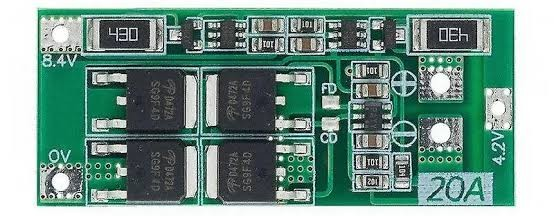
\includegraphics[width=0.75\textwidth]{Figures/2QHW/BMS_2S.jpg}
    \caption{The 2S 20A Lithium Battery Protection Module (BMS) utilized to actively balance and protect the stationary 18650 energy storage array.}
    \label{fig:bms_module}
\end{figure}

As shown in Figure \ref{fig:bms_module}, this specific module features heavy-duty protection MOSFETs and dedicated bleeding resistors for cell balancing.
\begin{itemize}
    \item \textbf{20A Continuous Discharge Rating:} Selecting a BMS with a massive 20A headroom ensures that the protection MOSFETs on the board do not become a thermal bottleneck or induce parasitic voltage drops ($V = I \times R_{BMS}$) during peak power extraction.
    \item \textbf{Active Balancing Capability:} In an off-grid solar context, battery strings are subjected to erratic charging cycles governed by cloud cover. The \textit{Balanced Version} of the BMS actively monitors the differential voltage across each individual 18650 cell. If one cell reaches its peak voltage prematurely, the BMS shunts the bypass current through bleeding resistors, allowing the lagging cell to continue charging. This indispensable feature guarantees synchronized state-of-charge (SoC).
    \item \textbf{Quad-Layer Protection:} The BMS autonomously enforces Over-Voltage Protection (OVP), Under-Voltage Protection (UVP), Over-Current Protection (OCP), and instant short-circuit isolation.
\end{itemize}

\subsubsection{Gate Driver Architecture and Galvanic Isolation}
\begin{itemize}
    \item \textbf{Selected Architecture (IR2111):} Features a single logic input ($IN$) and internally splits it into complementary outputs. Crucially, it features a \textbf{hardware-injected internal dead-time of 650 ns}. This provides an unbreakable, silicon-level physical block against shoot-through cross-conduction.
    \item \textbf{Selected Isolation (6N139):} A specialized high-speed optocoupler featuring a \textbf{Darlington-transistor output stage}. It allows the weak 5V logic signal from the microcontroller to deeply saturate the output transistor, effectively triggering the robust 12V gate drive stage with minimal nanosecond-level delay.
\end{itemize}

\subsection{Advanced Gate Drive Architecture and Hardware Logical Inversion}

\subsubsection{Miller Plateau Mitigation and Total Elimination of the Bootstrap Topology}
Driving the IRFP260N involves sweeping immense charge into its massive input capacitance ($C_{iss} \approx 3200\text{ pF}$). A \textbf{22 $\Omega$ series gate resistor ($R_G$)} was inserted alongside a \textbf{1N4148 fast-switching diode} to create an asymmetrical drive profile, ensuring $t_{off} \ll t_{on}$.

Furthermore, in a major design enhancement, \textbf{the traditional bootstrap circuit was entirely eliminated}. A bootstrap capacitor's voltage decays over time, mandating that the low-side switch periodically turns ON to recharge it ($D_{max} < 100\%$). By providing a dedicated, galvanically isolated 12V DC power supply directly to the floating channel ($V_B$ and $V_S$), the high-side MOSFET can be maintained in a continuous conduction state indefinitely, which is absolutely crucial for steady-state off-grid charging operation.

\subsubsection{Galvanic Isolation (6N139) and Hardware Logical Inversion}
The \textbf{6N139} high-speed optocoupler features a critical hardware characteristic in this specific wiring configuration: its \textbf{inherent logical inversion}. Because the internal phototransistor acts as an inverting switch, a HIGH logic signal from the MCU turns the optocoupler ON, which actively pulls the output node LOW. Consequently, as the original MCU Duty Cycle ($D$) increases, the actual effective voltage presented to the IR2111 gate driver decreases. 

\textbf{Software-Hardware Co-Design Solution:}
To counteract this hardware inversion without adding extra logic gate ICs (which consume PCB space and introduce delays), the hardware layout was maintained, and the correction was executed purely in software. If necessary, the embedded firmware could dynamically implement an inversion algorithm to guarantee perfectly linear control authority. However, in this implementation, the `TCCR1A` register was configured to naturally compensate for this behavior.

\newpage

\subsection{Microcontroller Firmware Architecture and Digital Control}
The physical hardware is tightly integrated with the embedded Microcontroller Unit (MCU) to form a robust closed-loop control nexus. Before executing complex Proportional-Integral (PI) loops, an \textbf{Open-Loop diagnostic firmware} was developed to validate the hardware integrity.

\subsubsection{Phase 1: Open-Loop Hardware Diagnostic Firmware}
To generate highly accurate PWM signals without blocking main loop execution, the MCU's internal 16-bit Timer1 hardware registers were manipulated directly. The open-loop code was set to a strict 50\% duty cycle at 10 kHz.

\begin{lstlisting}[language=C++, caption=Open-Loop Diagnostic Firmware (10kHz Timer1 PWM)]
/**
 * 50% Duty Cycle at 10kHz using Timer1
 * Pin 9 is the designated output
 */

const int PWM_PIN = 9;
const int TOP_PWM = 800; // Value that determines the 10kHz frequency

void setup() {
  pinMode(PWM_PIN, OUTPUT);

  // Stop timer for configuration and clear registers
  TCCR1A = 0;
  TCCR1B = 0;

  // Configure Fast PWM mode using ICR1 as the TOP value
  // COM1A1: Set pin to Clear OC1A on Compare Match (Non-Inverted at this stage)
  // WGM11 & WGM13: Set timer mode to Fast PWM
  TCCR1A = _BV(COM1A1) | _BV(WGM11); 
  TCCR1B = _BV(WGM13) | _BV(CS10);   
  
  ICR1 = TOP_PWM;                    
  
  // Set 50% Duty Cycle (50% of 800 = 400)
  OCR1A = 400; 
}

void loop() {
  // No code needed in the main loop; 
  // The timer executes autonomously in the background via hardware interrupts
}
\end{lstlisting}

\newpage

\subsubsection{Phase 2: Closed-Loop PI Control and Fixed-Point Arithmetic Integration}
Once the open-loop phase proved the power stage could switch safely at 10 kHz, the firmware was upgraded to a fully calibrated Proportional-Integral (PI) closed-loop controller. 

As theoretically established in Section 4.1.2.6, the PI controller was discretized via the Bilinear Z-Transform. This mathematical transformation yields the discrete coefficients (\texttt{B0\_i}, \texttt{B1\_i}, and \texttt{A1\_i}) utilized in the firmware, ensuring a strict correlation between the theoretical continuous-time system and the digital discrete-time hardware.

Furthermore, realizing the computational limitations of an 8-bit MCU operating at high switching frequencies, the control algorithm was engineered utilizing \textbf{Fixed-Point Arithmetic} via the \texttt{GEN\_SCALE 131072L} variable. By eliminating slow floating-point operations and relying on bit-shifting (e.g., \texttt{>> SC\_B}), the MCU executes the PI calculations well within the 10 kHz hardware interrupt (\texttt{ISR(TIMER1\_OVF\_vect)}) overhead without blocking the main system. The success of this inner current loop (Constant Current - CC) directly validates the foundational requirement for the comprehensive CC-CV charging architecture extensively evaluated in Chapter 5.

\begin{lstlisting}[language=C++, caption=Advanced Fixed-Point PI Controller using Timer1 ISR]
#define     SC_B        17                                    //number of bits for fixed point scaling
#define     GEN_SCALE   131072L                               //2^SC_B

#define     dr_min      (int32_t)(0.0f*GEN_SCALE)             //minimum scaled duty cycle
#define     dr_max      (int32_t)(1.0f*GEN_SCALE)            //maximum scaled duty cycle

#define     I_SCALE     (int32_t)(0.005f*GEN_SCALE)    //scaled current sensor gain

#define     OFFSET     (int32_t)(22.643f*GEN_SCALE)    //sensor offset 520/1024*5.12

#define     sensitivity      (int32_t)(0.185f*GEN_SCALE)            //sensor sensitivity 185mV/A

#define     Io_ref      (int32_t)(0.3f*GEN_SCALE)            //output current reference

#define      B0_i    (int32_t)(0.0094875*GEN_SCALE)
#define      B1_i    (int32_t)(-0.0076936*GEN_SCALE)
#define      A1_i    (int32_t)(1*GEN_SCALE)


#define     MAX_DUTY    1599L                                  //True maximum duty cycle


void PWM_TMR_INIT();    //PWM initialiazation function 
void ADC_INIT();        //ADC initialization function 
int32_t SAMPLE_IO();    //output current sampling function 


int32_t GEN_CTRL_PI(int64_t m_r[], int32_t e_r[], int32_t ref_C, int32_t adc_C,
                    int32_t A1_g, int32_t B0_g, int32_t B1_g,
                 int32_t lo_limit, int32_t up_limit);

void BUCK_ICNTRL_PI(void);      //PI current control


int64_t m_i[4] = {0};           //current control array
int32_t e_i[4] = {0};           //current error array

int32_t Io = 0;                 //output current


void setup(){
  PWM_TMR_INIT();               //Initialize the pwm 
  ADC_INIT();                   //Initialize the adc 

  DDRB |= (1 << DDB5);          //Initialize PORTB5 as a digital output
}

void loop(){
}

ISR(TIMER1_OVF_vect){
  PORTB |= (1 << PORTB5);     //set pin PORTB5

  BUCK_ICNTRL_PI();           //Execute PI current control
  PORTB &= ~(1 << PORTB5);    //clear pin PORTB5
}

void PWM_TMR_INIT(){
  //Clear the TMR1 control registers
  TCCR1A = 0;
  TCCR1B = 0;
  TCNT1 = 0;

  TCCR1A |= (1 << COM1A1);    //Set up in non-inverting mode

  //Set up in fast pwm mode
  TCCR1A |= (1 << WGM11);
  TCCR1B |= (1 << WGM12);
  TCCR1B |= (1 << WGM13);
  
  //Set a prescale ratio of 1
  TCCR1B |= (1 << CS10);

  //PWM frequency of 10kHz
  ICR1 = 1599;

  //Set up pin D9 as an output
  pinMode(9, OUTPUT);

  //Set up tmr1 interrupt
  TIMSK1 |= (1 << TOIE1);
  sei();
}

void ADC_INIT(){
  //Set up adc current reference
  ADMUX &= ~(1 << REFS1);
  ADMUX |= (1 << REFS0);

  //adc clock prescale 16
  ADCSRA |= (1 << ADPS2);
  ADCSRA &= ~(1 << ADPS1);
  ADCSRA &= ~(1 << ADPS0);

  //enable the adc
  ADCSRA |= (1 << ADEN);
}

int32_t SAMPLE_IO(){
  //use channel ADC0 - pin A0
  ADMUX &= ~(1 << MUX3);
  ADMUX &= ~(1 << MUX2);
  ADMUX &= ~(1 << MUX1);
  ADMUX &= ~(1 << MUX0);

  ADCSRA |= (1 << ADSC);        //set the ADSC bit
  while(ADCSRA & (1 << ADSC));  //poll the ADSC bit

  return ADC;                   //return the ADC conversion result
}

int32_t GEN_CTRL_PI(int64_t m_r[], int32_t e_r[], int32_t ref_C, int32_t adc_C,
                    int32_t A1_g, int32_t B0_g, int32_t B1_g,
                    int32_t lo_limit, int32_t up_limit){

    m_r[0] = (A1_g*m_r[1] + B0_g*e_r[0] + B1_g*e_r[1])>>SC_B;   //compute the PI output control step


    //limit the control output
    if(m_r[0] < lo_limit){
        m_r[0] = lo_limit;
    }
    else if(m_r[0] > up_limit){
        m_r[0] = up_limit;
    }

    //return the control output
    return m_r[0];
}

void BUCK_ICNTRL_PI(void){
    int32_t pwm;
    int32_t numerator = SAMPLE_IO() * I_SCALE - OFFSET;
    Io = ((numerator << SC_B) / sensitivity);
    //Compute the output current
    //Io = (SAMPLE_IO()*I_SCALE - OFFSET) / sensitivity;
e_i[0] = Io_ref - Io;   //compute the output current error
 //compute the true pwm duty cycle using a PI controller
    pwm = (MAX_DUTY*GEN_CTRL_PI(m_i, e_i, Io_ref, Io,
                                  A1_i, B0_i, B1_i,
                                  dr_min, dr_max))>>SC_B;
    m_i[1] = m_i[0];        //update the previous control output
    e_i[1] = e_i[0];        //update the previous error

    //write the pwm to the output capture register
    OCR1A = pwm;
}
\end{lstlisting}

\newpage

\subsection{Pre-Fabrication Breadboard Prototyping}
Prior to committing the schematic to a fabricated PCB, rigorous empirical validation was executed on a prototyping breadboard. This phased approach allowed for safe, iterative testing of the firmware and gate drive parameters.

\begin{figure}[H]
    \centering
    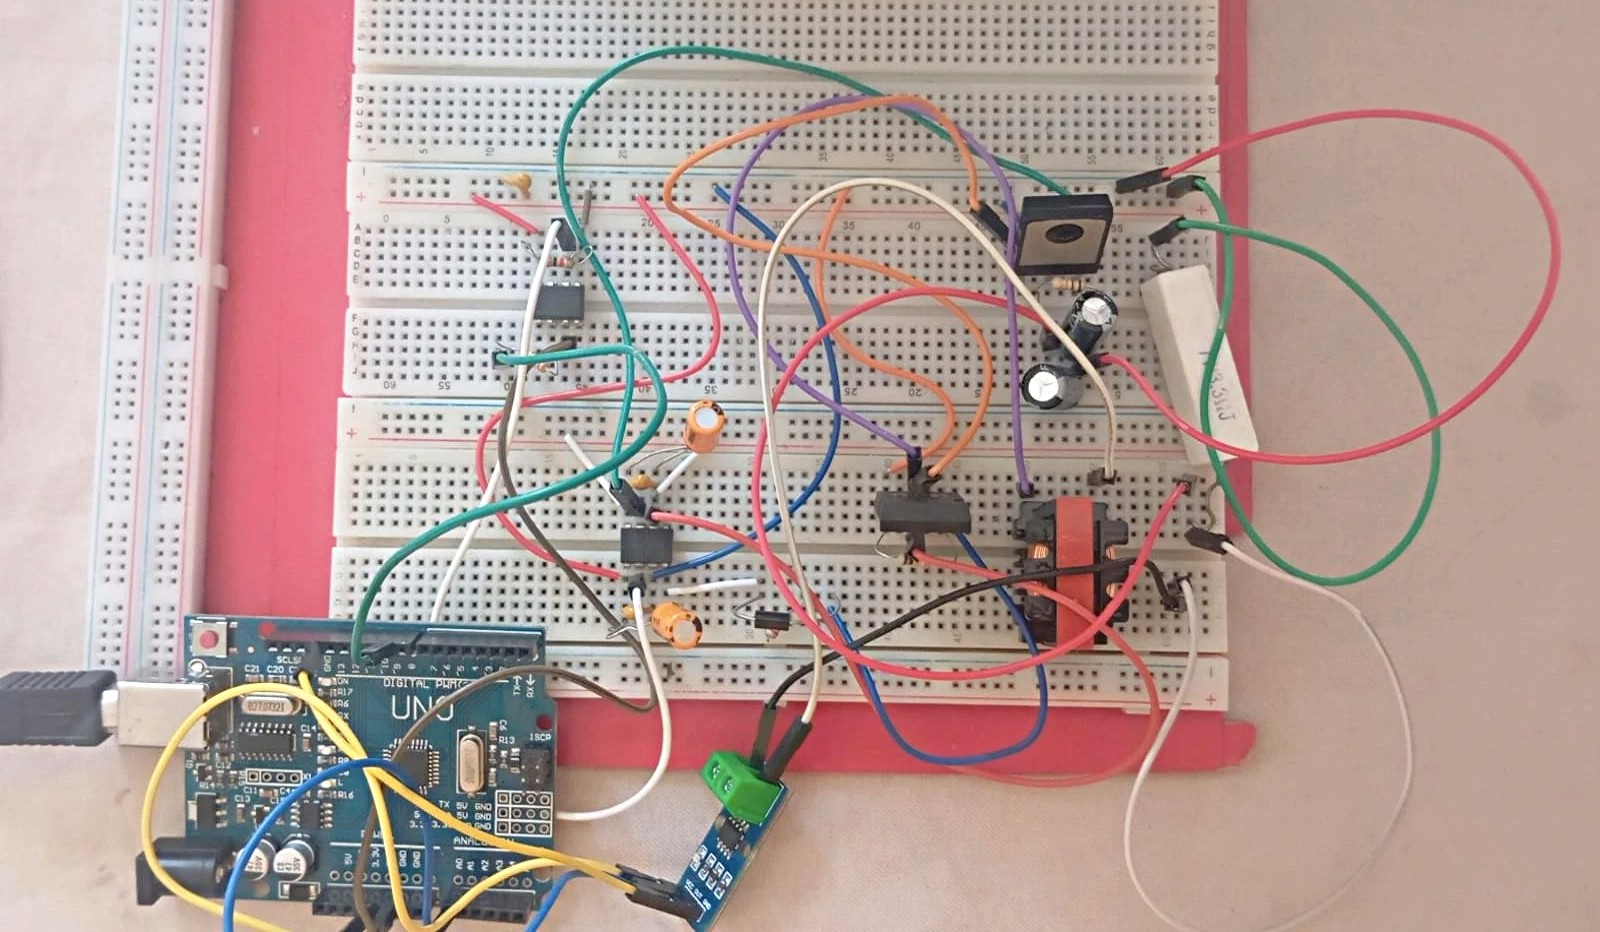
\includegraphics[width=0.85\textwidth]{Figures/2QHW/breadboard_passive.jpg}
    \caption{Phase 1: Breadboard prototype driving a $3.3\text{ }\Omega$ passive load. The configuration safely dissipates power as heat while allowing probing of the gate drive signals.}
    \label{fig:breadboard_passive}
\end{figure}

As shown in Figure \ref{fig:breadboard_passive}, a heavy-duty $3.3\text{ }\Omega$, $7\text{ W}$ wire-wound resistor was employed in conjunction with the primary switching MOSFET. This phase successfully confirmed that the MCU's PWM signals were accurately triggering the optocouplers without risking battery chemistry.

\begin{figure}[H]
    \centering
    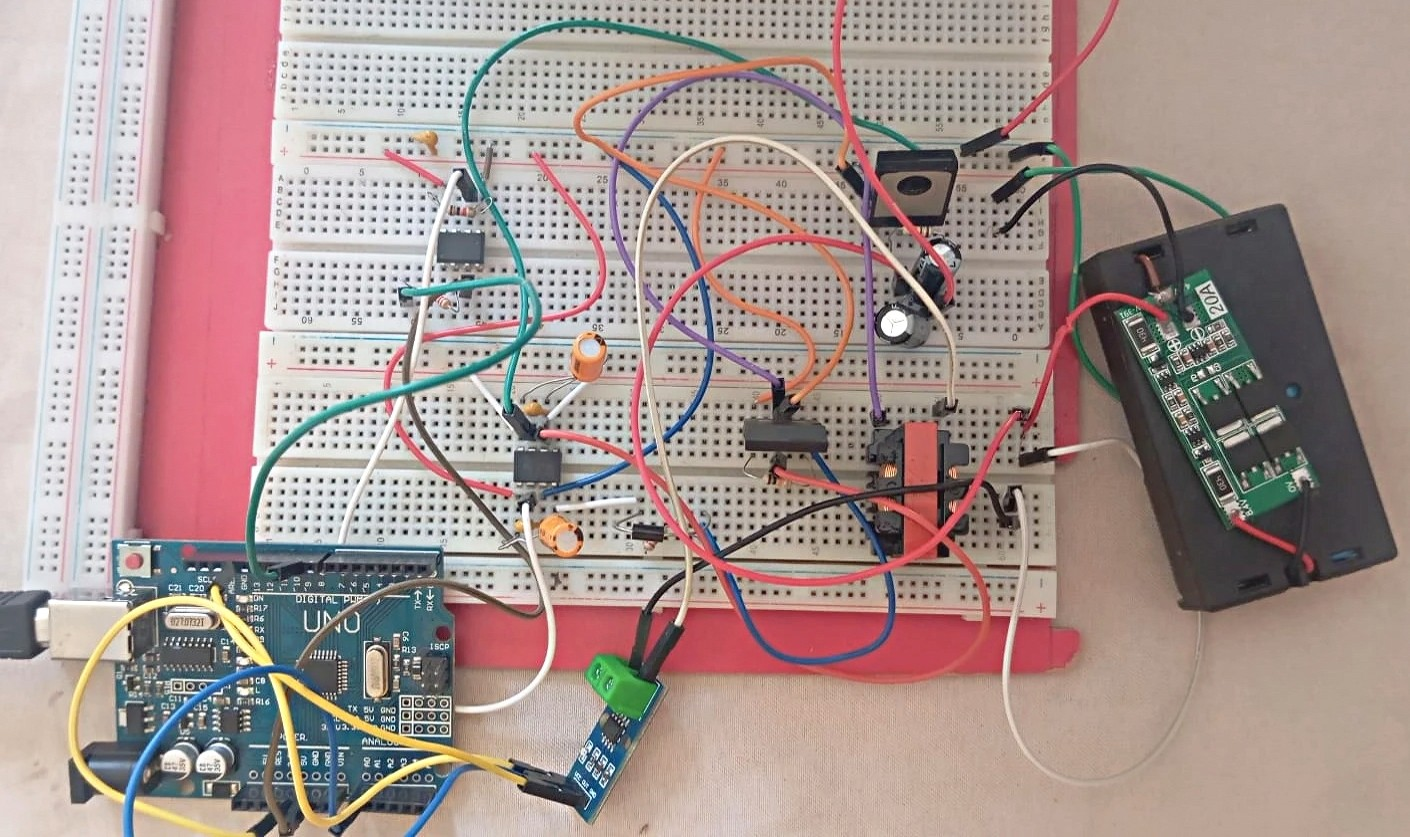
\includegraphics[width=0.85\textwidth]{Figures/2QHW/breadboard_battery.jpg}
    \caption{Phase 2: Breadboard prototype executing active charging of the 7.4V lithium-ion battery pack, validating the bidirectional energy transfer topology.}
    \label{fig:breadboard_battery}
\end{figure}

Following the passive load success, the actual 2S lithium-ion battery pack was integrated (Figure \ref{fig:breadboard_battery}). The transition to an active load introduced significant back-EMF and dynamic resistance variables. This critical testing phase allowed for the meticulous tuning of the PI controller's $K_p$ and $K_i$ gains, ensuring that the charging current stabilized at the targeted reference without inducing dangerous overshoot oscillations in the battery pack.

\subsection{Schematic Design, PCB Layout, and EMC Engineering}
Having validated the architecture on the breadboard, translating the circuit into a robust physical Printed Circuit Board (PCB) required extreme adherence to high-power routing standards to permanently mitigate stray inductance ($L_{\text{stray}}$).

\begin{figure}[H]
    \centering
    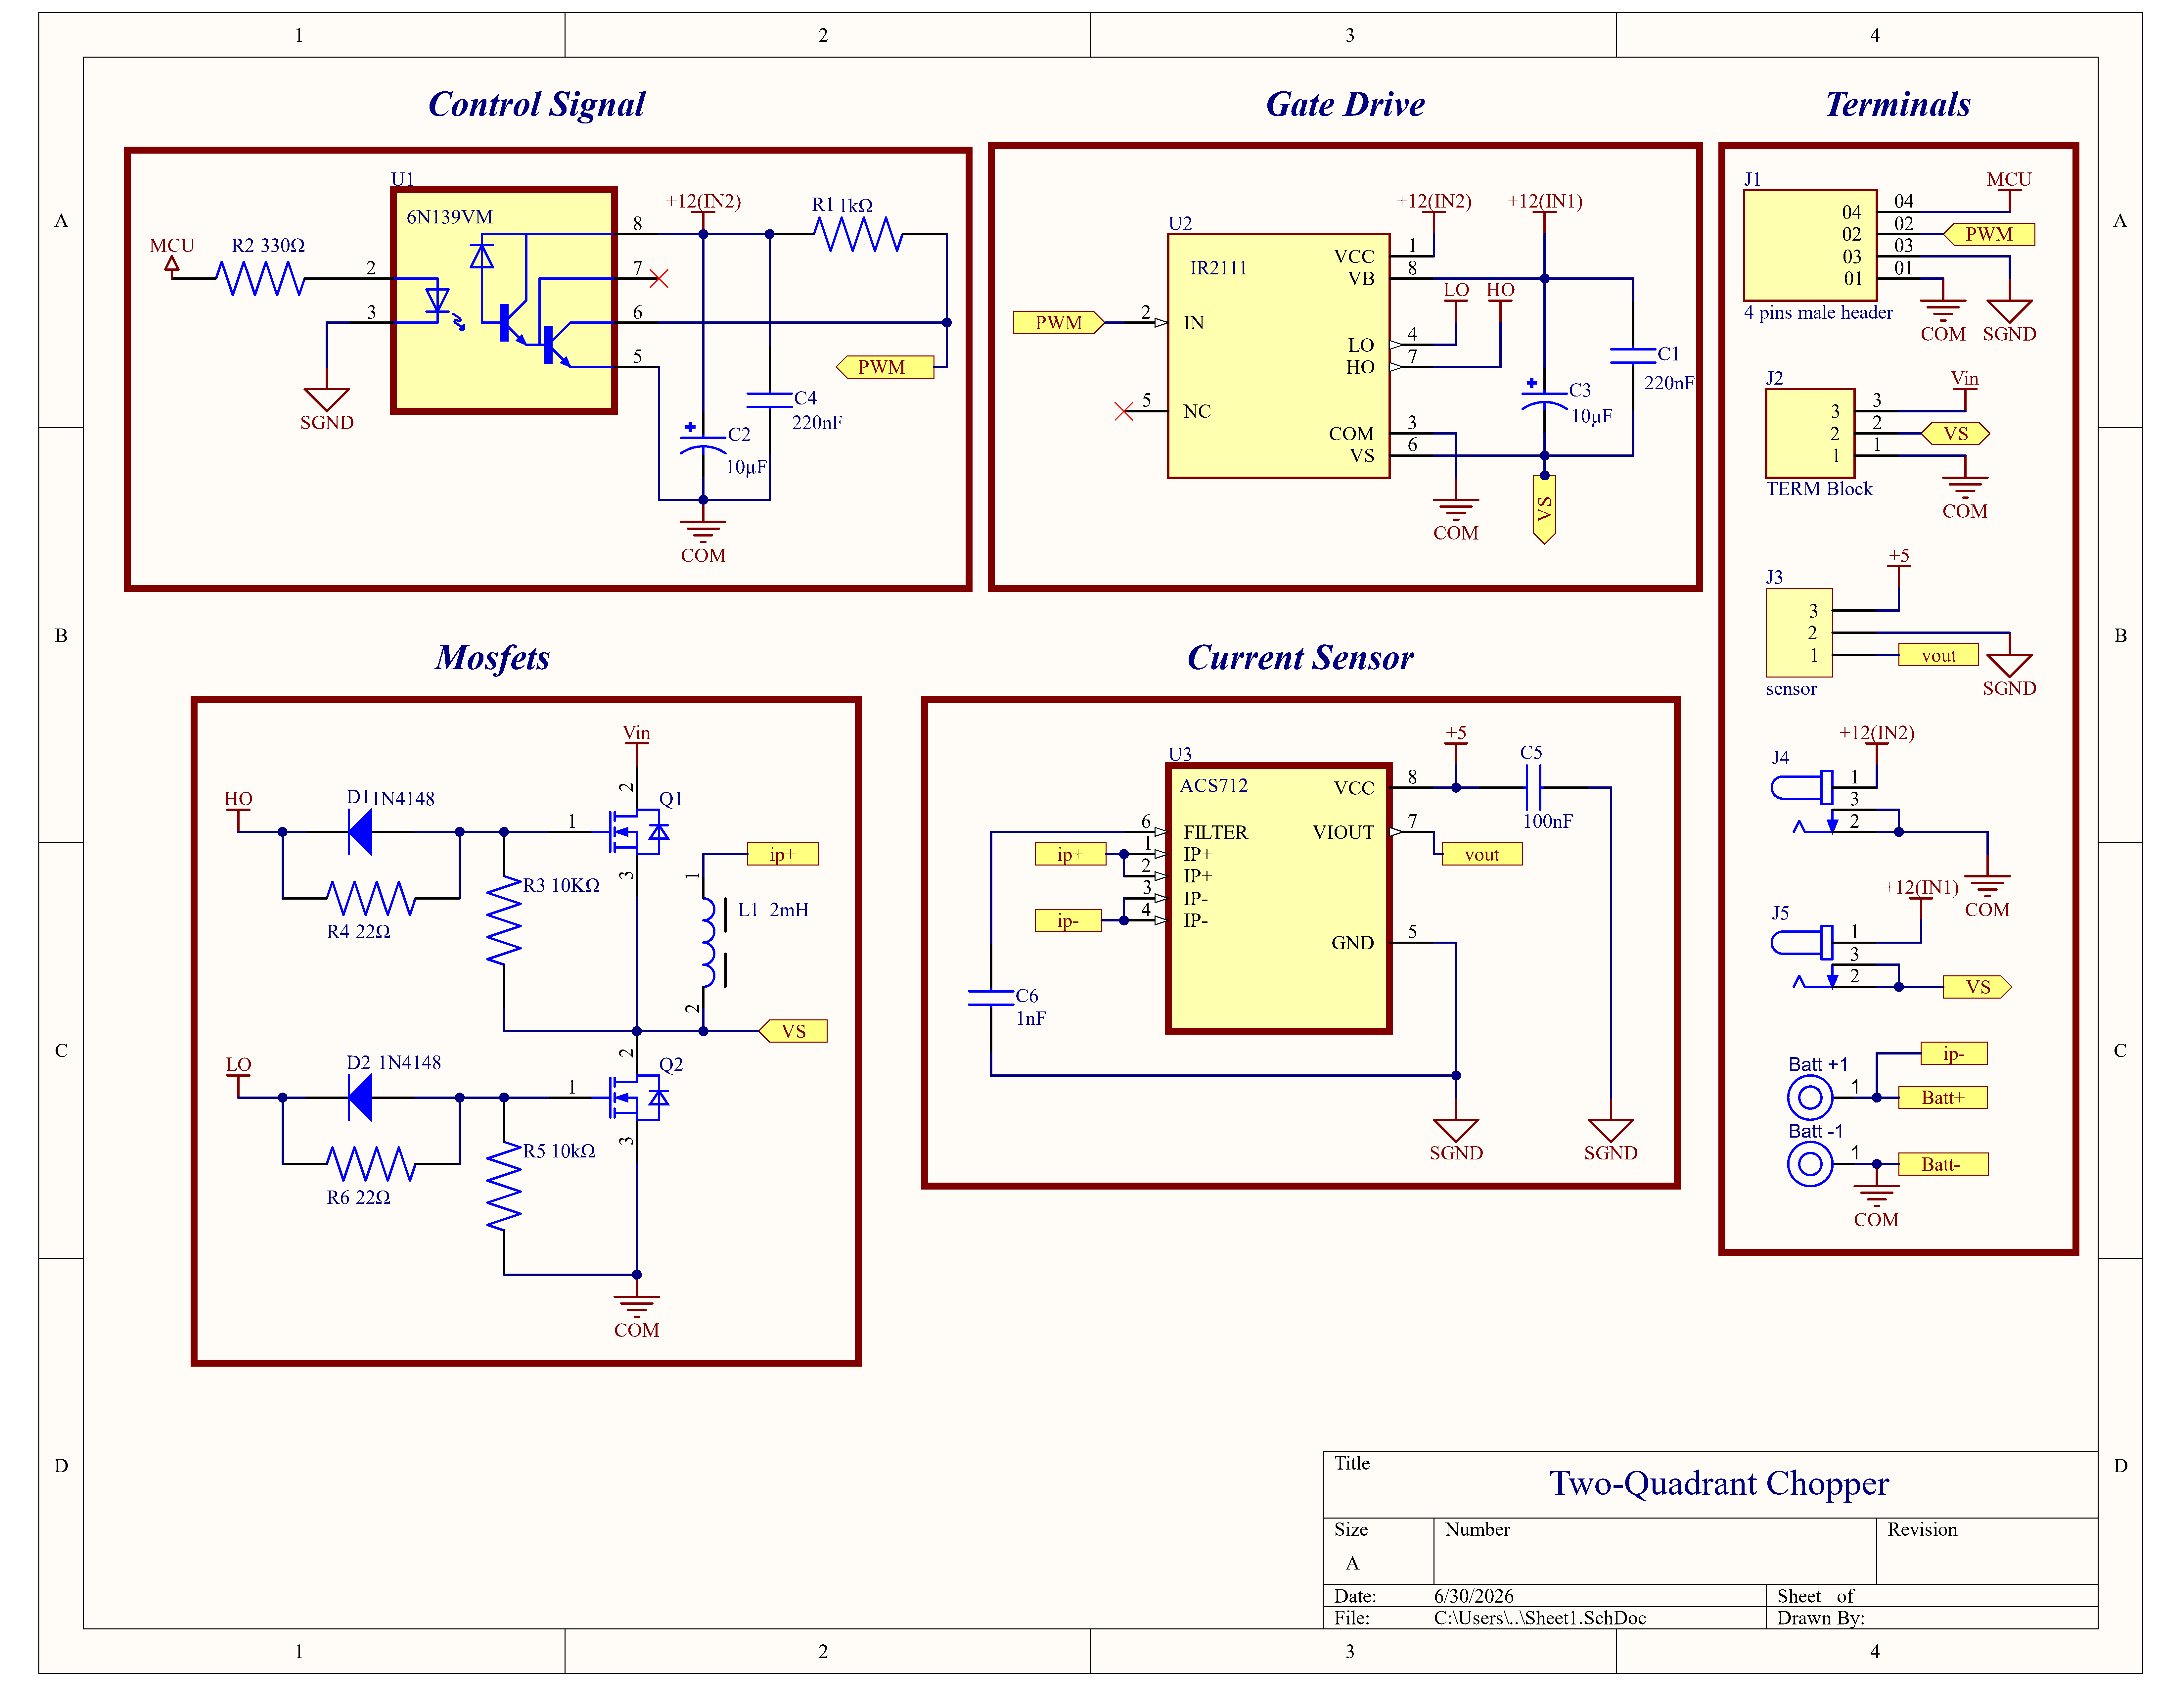
\includegraphics[width=1\textwidth]{Figures/2QHW/schematic.png}
    \caption{Complete electrical schematic of the Two-Quadrant Chopper detailing the isolated IR2111 gate drive topology, 6N139 galvanic isolation barrier, and ACS712 current sensing matrix.}
    \label{fig:full_schematic}
\end{figure}

The foundation of the physical design relies entirely on the electrical schematic depicted in Figure \ref{fig:full_schematic}. To guarantee signal integrity in a noisy, high-frequency switching environment, IPC-2221 trace width standards were applied. The power-carrying nodes ($V_{in}, VS, COM$) were routed using massive copper polygons rather than standard tracks, ensuring the DC trace resistance is kept strictly negligible.

\begin{figure}[H]
    \centering
    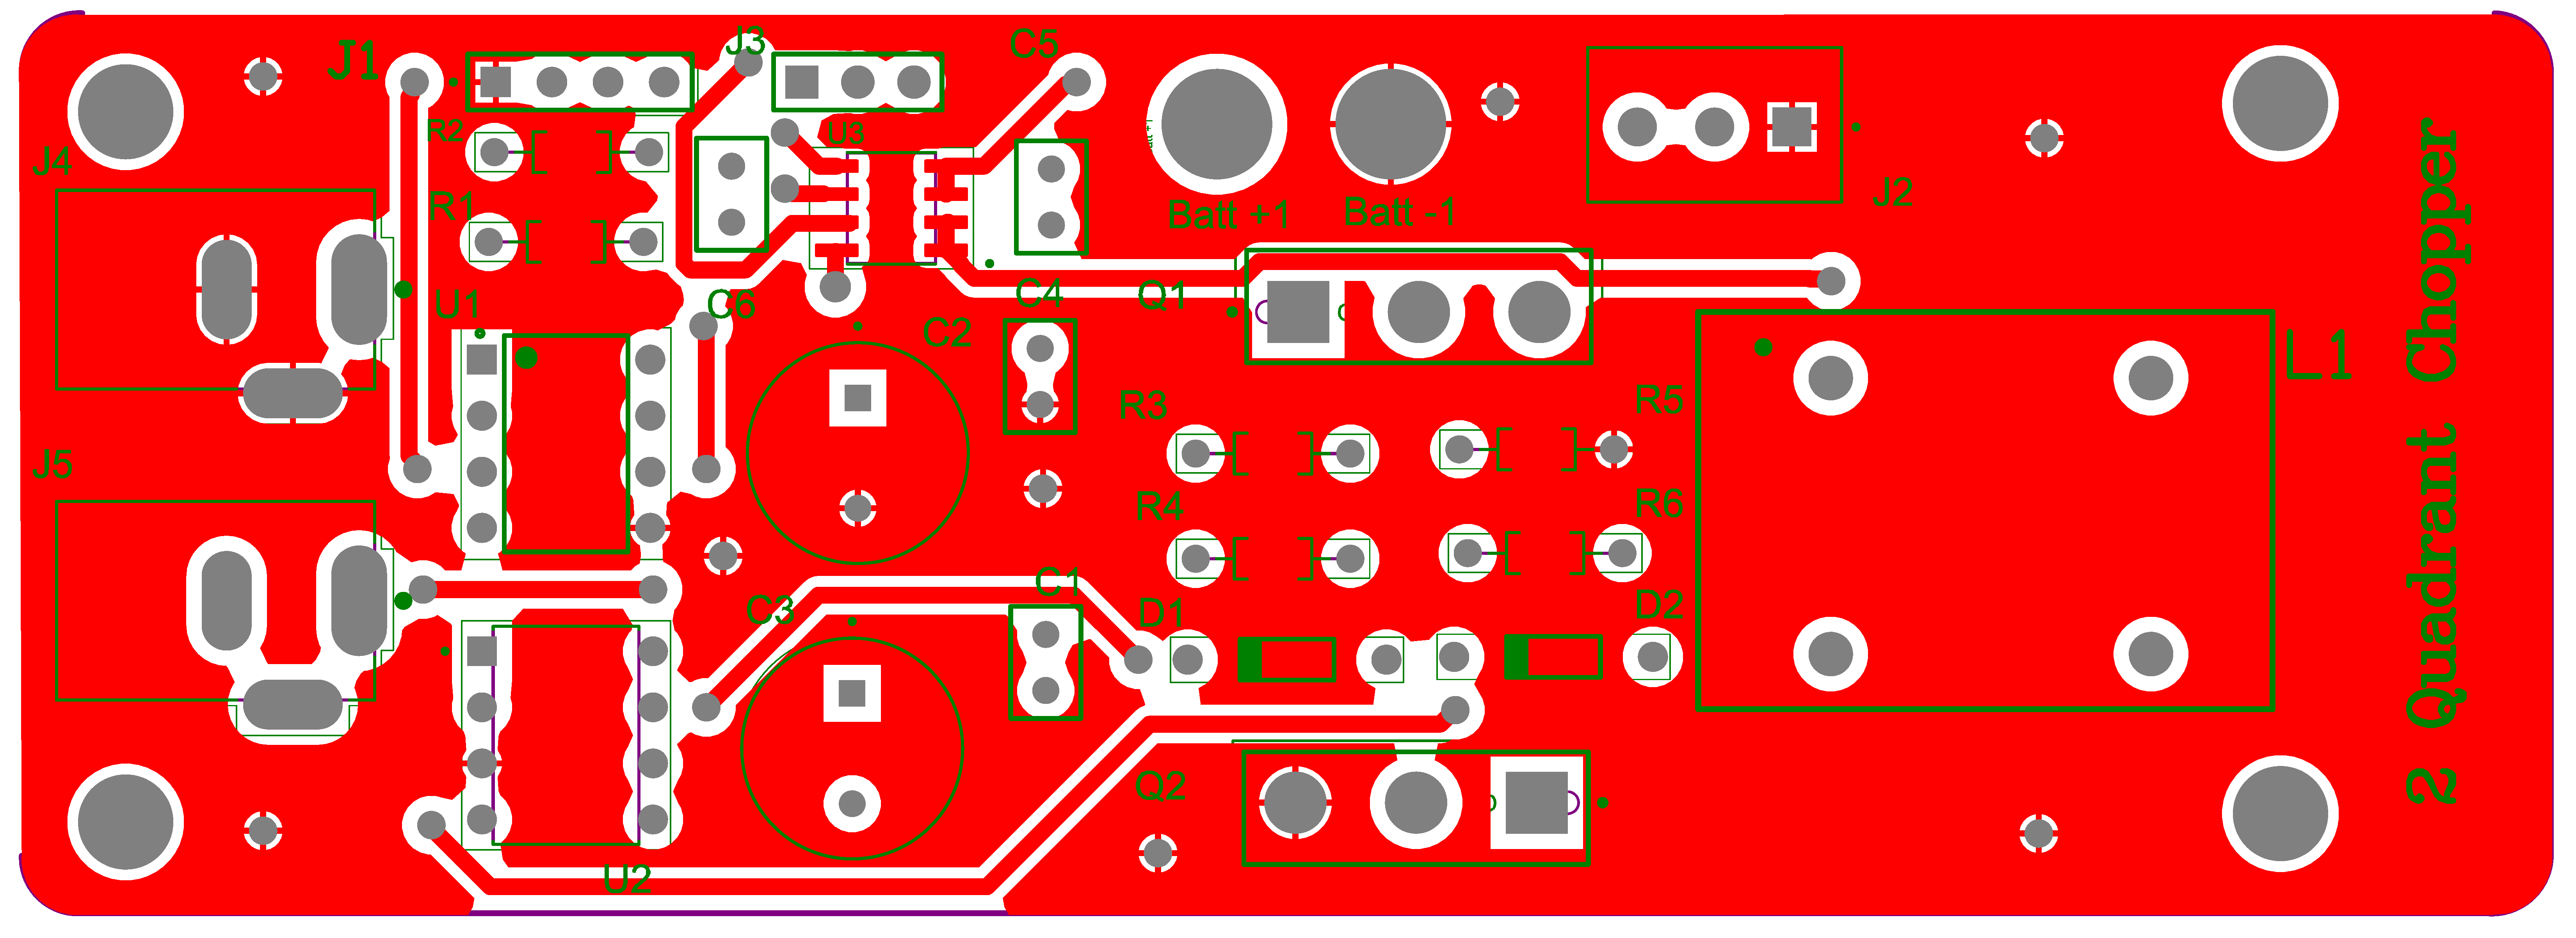
\includegraphics[width=0.85\textwidth]{Figures/2QHW/pcb_top.png}
    \caption{Top Copper Layer (Red) Layout, illustrating massive polygon pours for high-current nodes to drastically reduce Equivalent Series Resistance (ESR).}
    \label{fig:pcb_top}
\end{figure}

As illustrated in the top layer routing above (Figure \ref{fig:pcb_top}), the sheer surface area of these polygons provides excellent thermal dissipation capabilities without the need for auxiliary copper busbars. Following the top-layer high-current routing, the bottom layer strictly separates the Signal Ground (SGND) from the noisy Power Ground (PGND).

\begin{figure}[H]
    \centering
    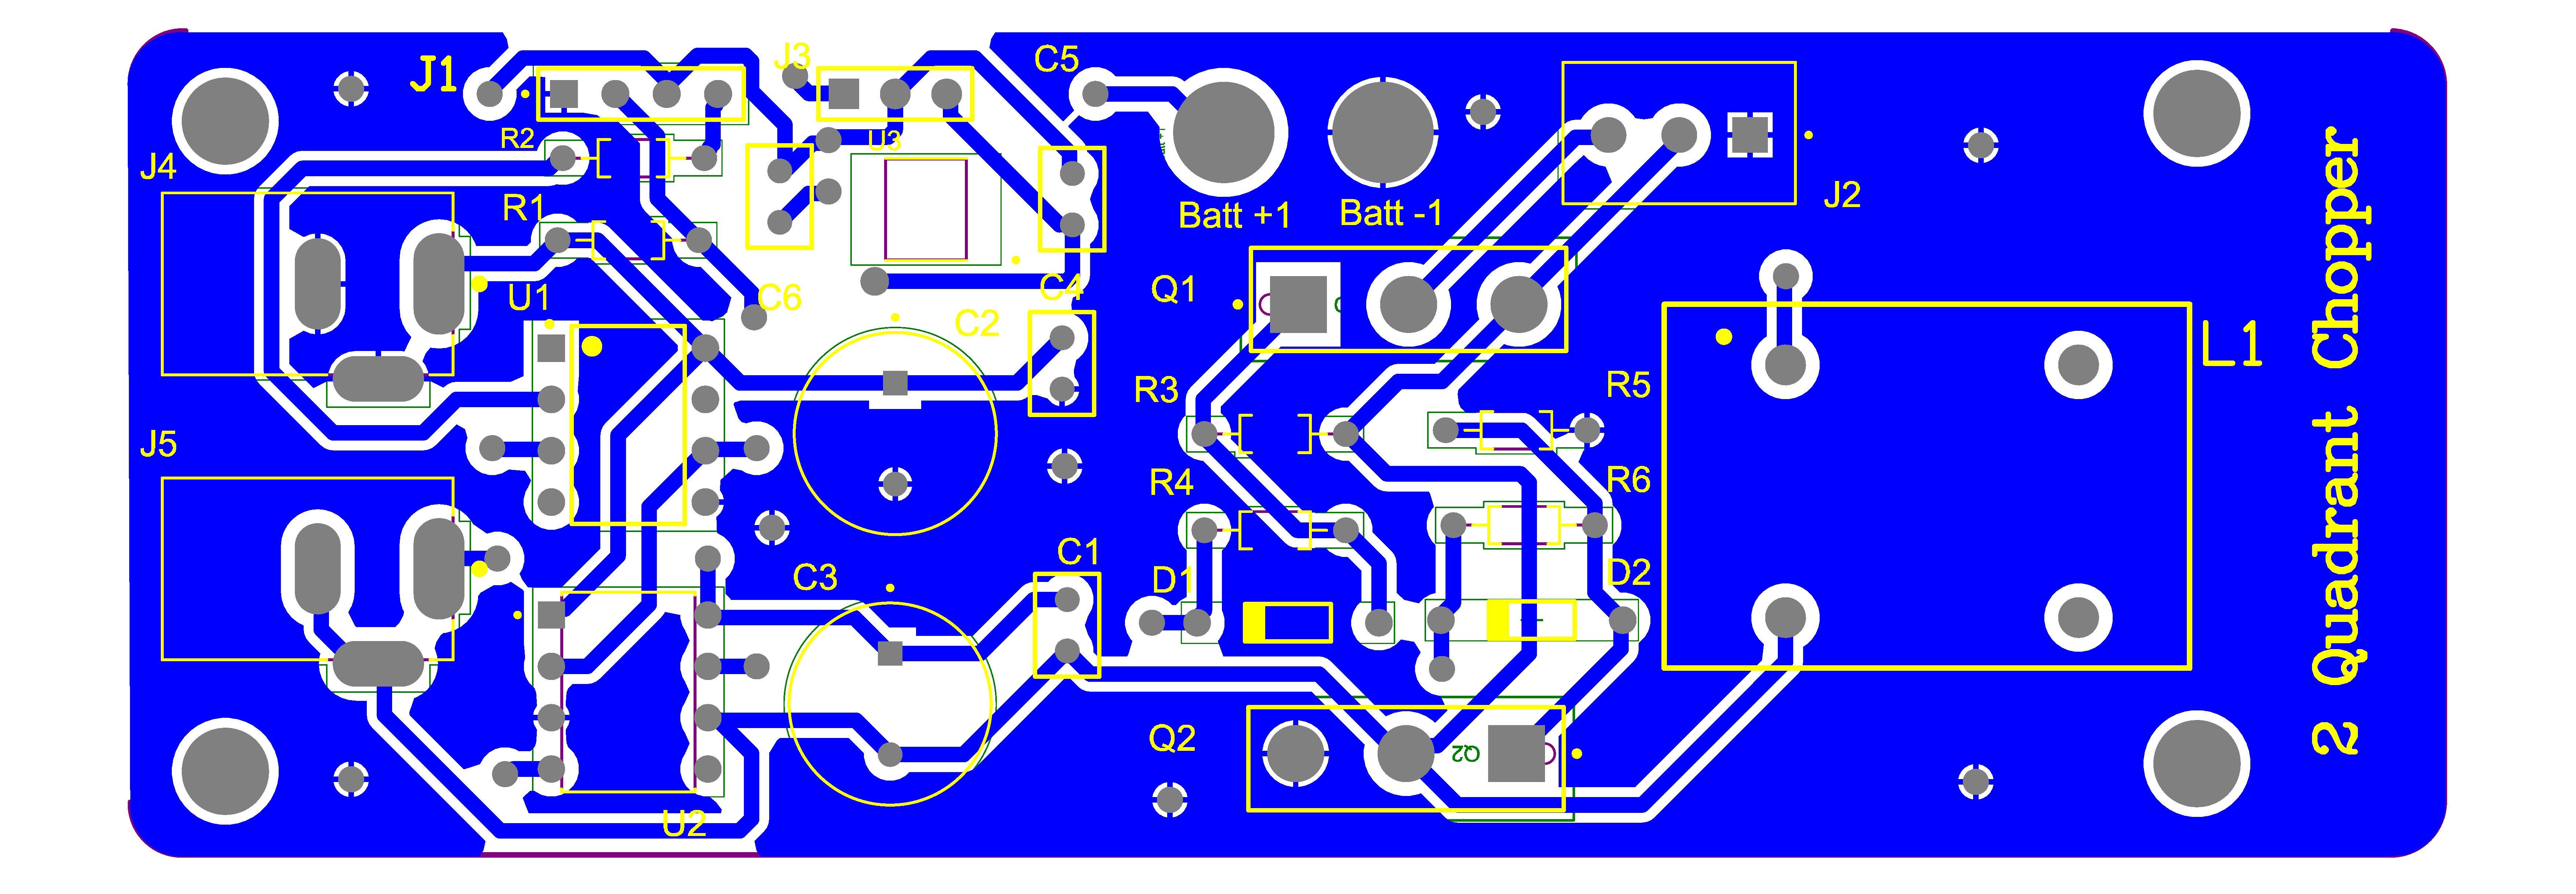
\includegraphics[width=0.85\textwidth]{Figures/2QHW/pcb_bottom.png}
    \caption{Bottom Copper Layer (Blue) Layout, demonstrating the strict physical separation of PGND and SGND. A single "Star Ground" connection definitively prevents common-impedance EMI coupling.}
    \label{fig:pcb_bottom}
\end{figure}

By keeping the PGND and SGND planes distinct and localized (Figure \ref{fig:pcb_bottom}), massive high-current return loops are actively prevented from polluting the delicate ADC control logic. Moving beyond 2D routing, ensuring precise mechanical integration required comprehensive 3D CAD analysis.

\begin{figure}[H]
    \centering
    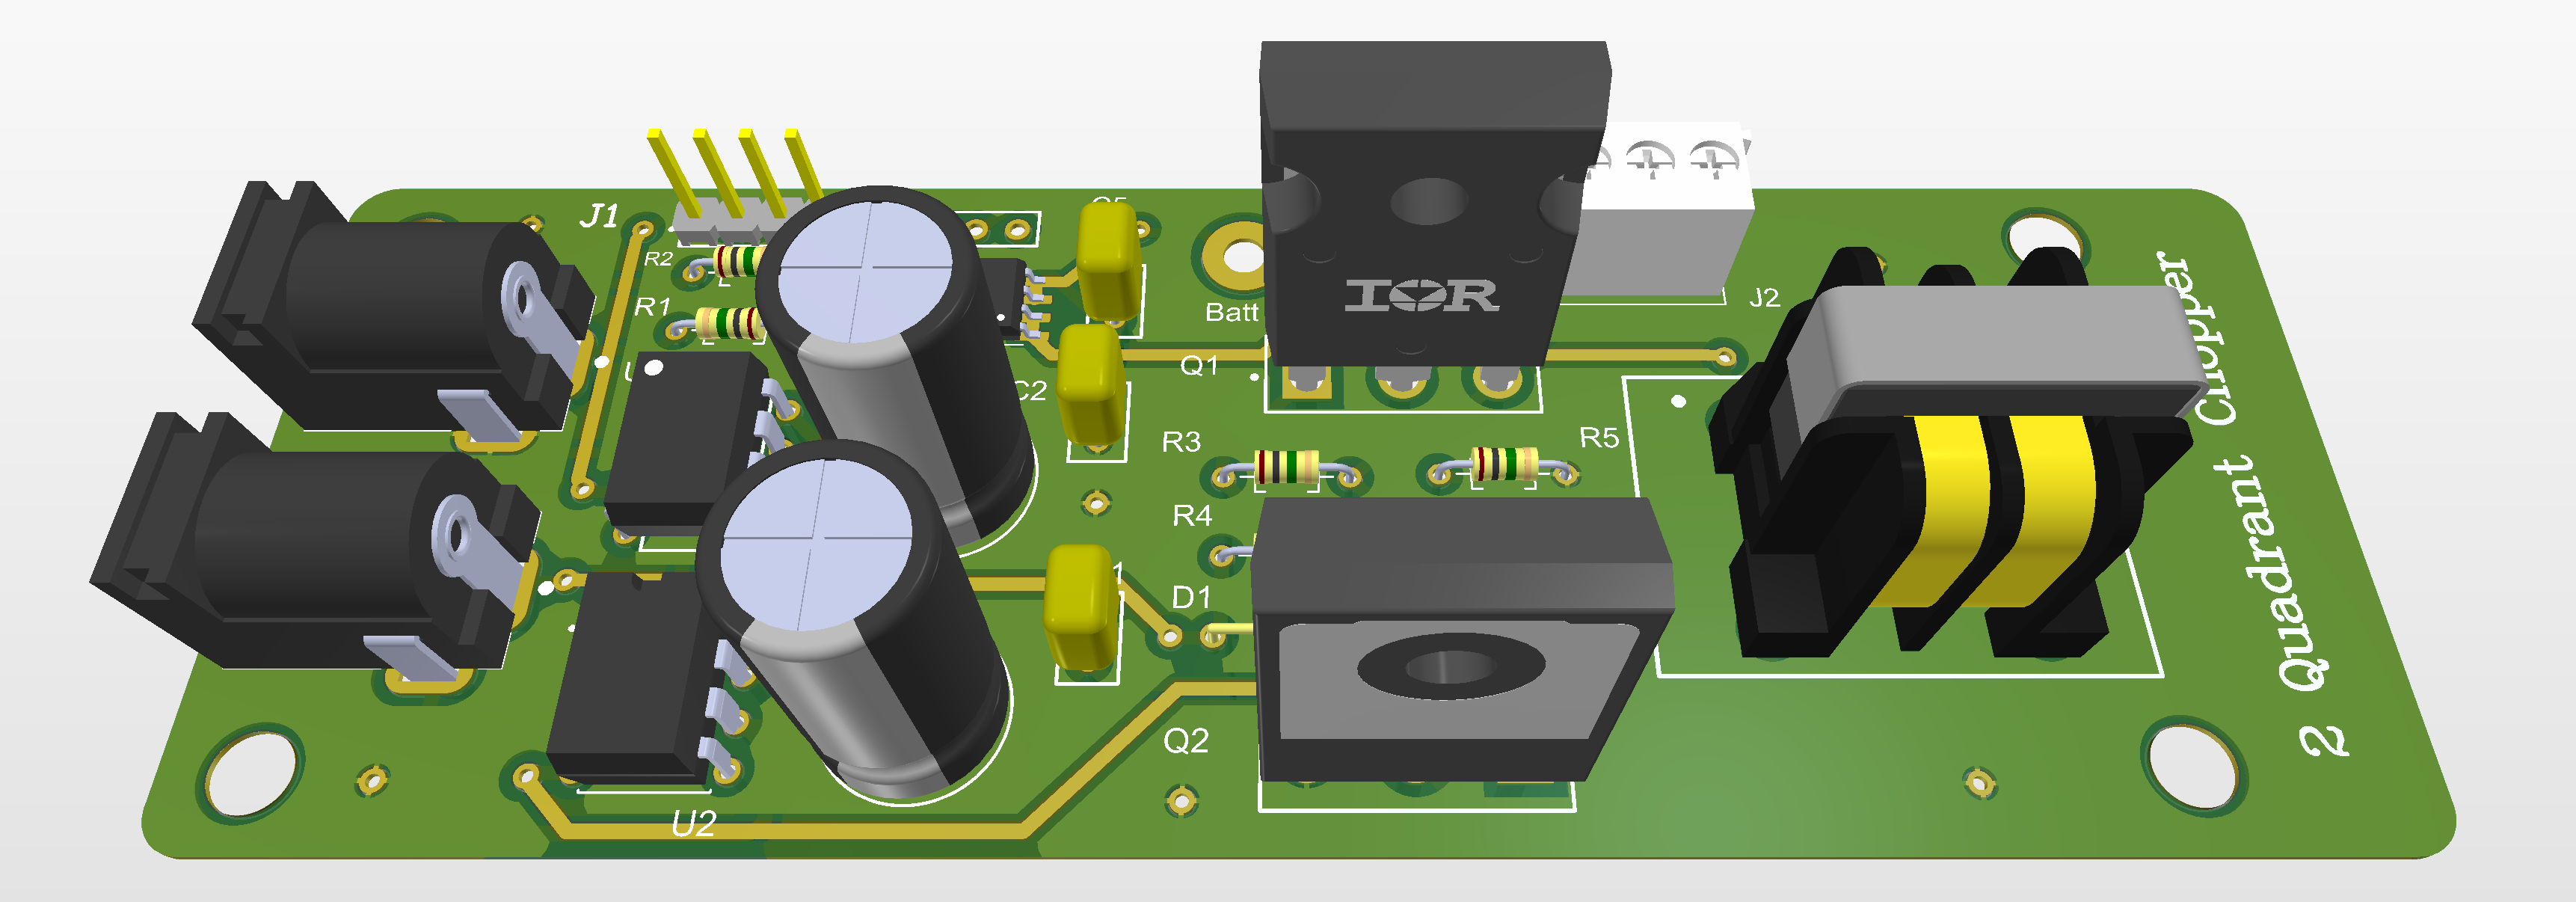
\includegraphics[width=0.85\textwidth]{Figures/2QHW/pcb_3d_isometric.png}
    \caption{Isometric 3D Render: Validating component heights, volumetric clearance, and overall mechanical viability of the PCB assembly.}
    \label{fig:pcb_3d_iso}
\end{figure}

The isometric render (Figure \ref{fig:pcb_3d_iso}) confirms that the IRFP260N (TO-247) MOSFETs are strategically placed at the perimeter of the board, ensuring unobstructed convective airflow. 

\begin{figure}[H]
    \centering
    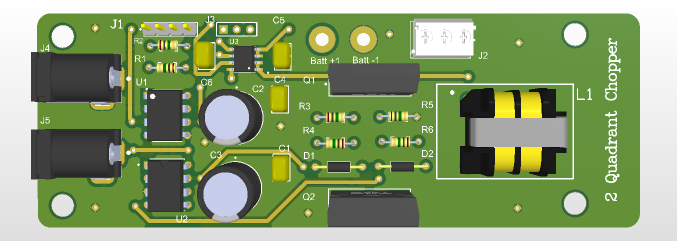
\includegraphics[width=0.85\textwidth]{Figures/2QHW/pcb_3d_top.png}
    \caption{Top Orthogonal 3D View: Highlighting terminal block accessibility, sensor positioning, and the physical distance defining the galvanic isolation barrier.}
    \label{fig:pcb_3d_top}
\end{figure}

The top orthogonal view (Figure \ref{fig:pcb_3d_top}) reveals that the physical distance between the 12V/7.4V power tracks and the 5V MCU control logic is visibly maximized, adhering to standard creepage safety protocols. 

\begin{figure}[H]
    \centering
    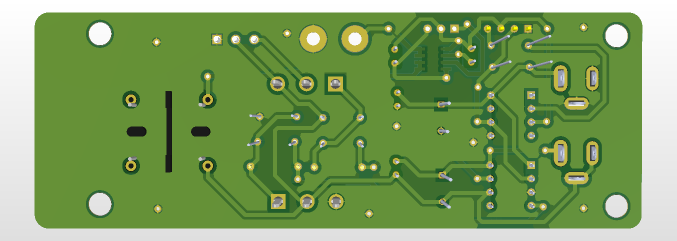
\includegraphics[width=0.85\textwidth]{Figures/2QHW/pcb_3d_bottom.png}
    \caption{Bottom Orthogonal 3D View: Verifying solder mask application, via tenting, and through-hole pin clearances.}
    \label{fig:pcb_3d_bottom}
\end{figure}

Finally, the bottom 3D view (Figure \ref{fig:pcb_3d_bottom}) is utilized to validate the manufacturing constraints. It confirms proper via tenting and ensures adequate annular ring clearance to prevent accidental solder bridging.

\begin{figure}[H]
    \centering
    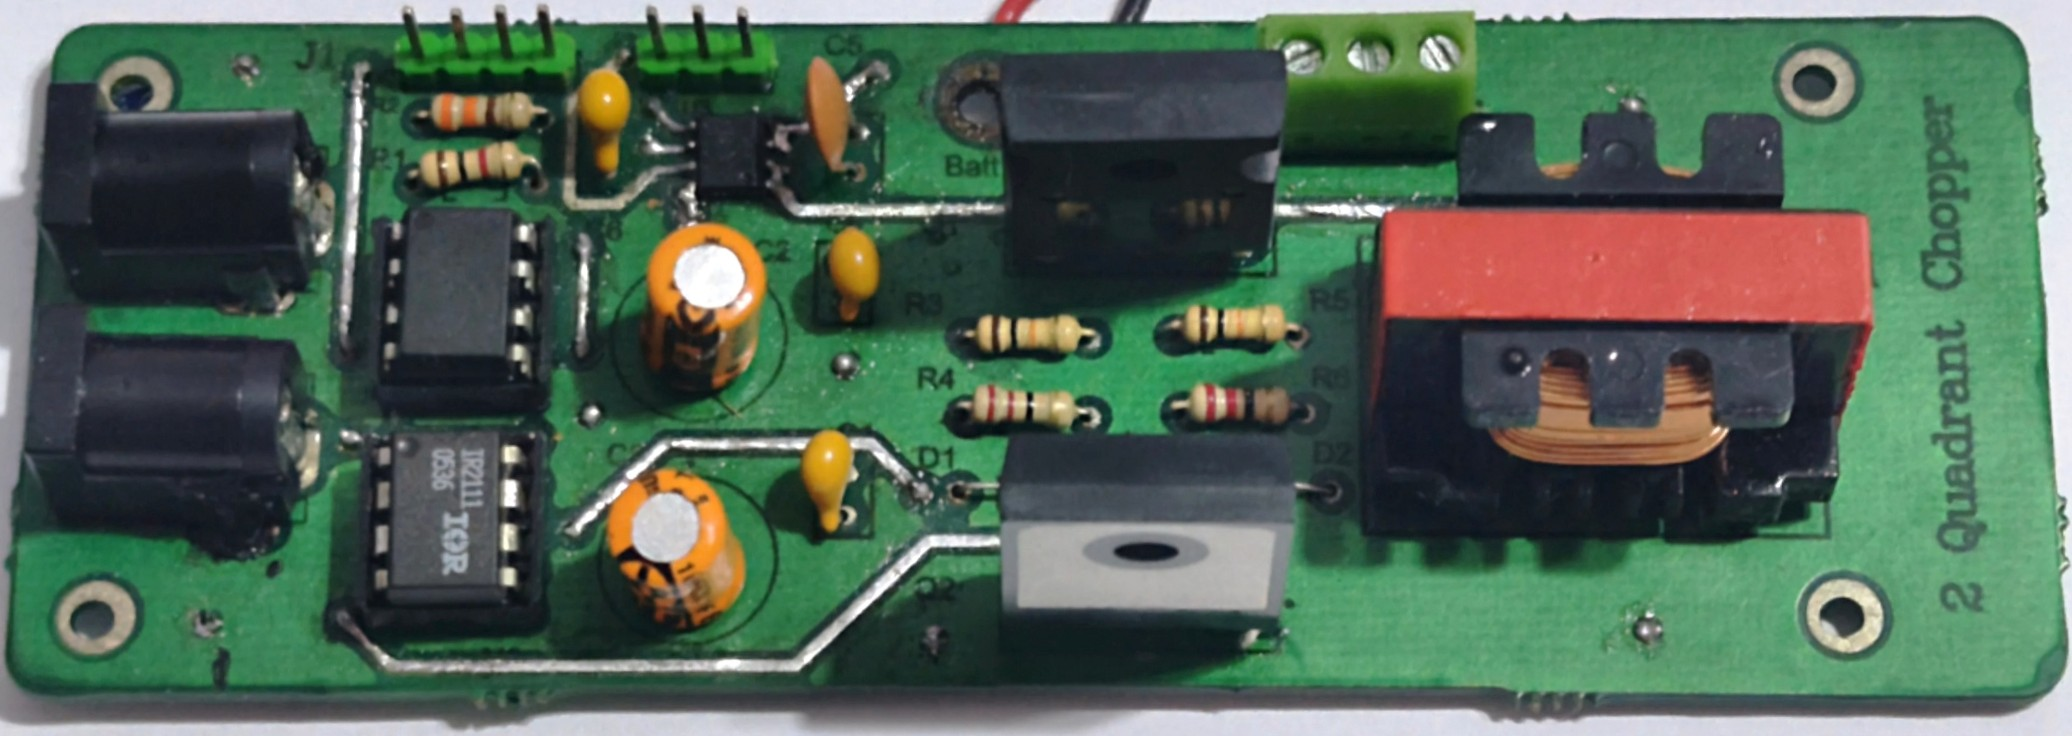
\includegraphics[width=0.85\textwidth]{Figures/2QHW/pcb_actual_board.jpg}
    \caption{The fully assembled and soldered physical PCB prototype, showcasing the integration of the 2 mH inductor, TO-247 MOSFETs, and terminal connectors.}
    \label{fig:pcb_actual}
\end{figure}

Following fabrication, the physical assembly and soldering of the board (Figure \ref{fig:pcb_actual}) required precise thermal management to avoid damaging the sensitive semiconductor junctions. The completed board reflects a robust, industrial-grade layout capable of sustaining continuous currents.

\subsection{Experimental Validation and Empirical Signal Analysis}
Prior to committing to the final operation, rigorous empirical validation was executed using the \textbf{Hantek DSO4254B Digital Storage Oscilloscope}.

\subsubsection{Test 1: Open-Loop 10kHz PWM Validation (Duty Cycle Sweep)}
To empirically verify the Timer1 hardware registers and explicitly demonstrate the inverting nature of the optocoupler, a duty cycle sweep was conducted. First, the MCU was programmed to output a 50\% Duty Cycle ($D=0.5$).

\begin{figure}[H]
    \centering
    \begin{subfigure}[b]{0.48\textwidth}
        \centering
        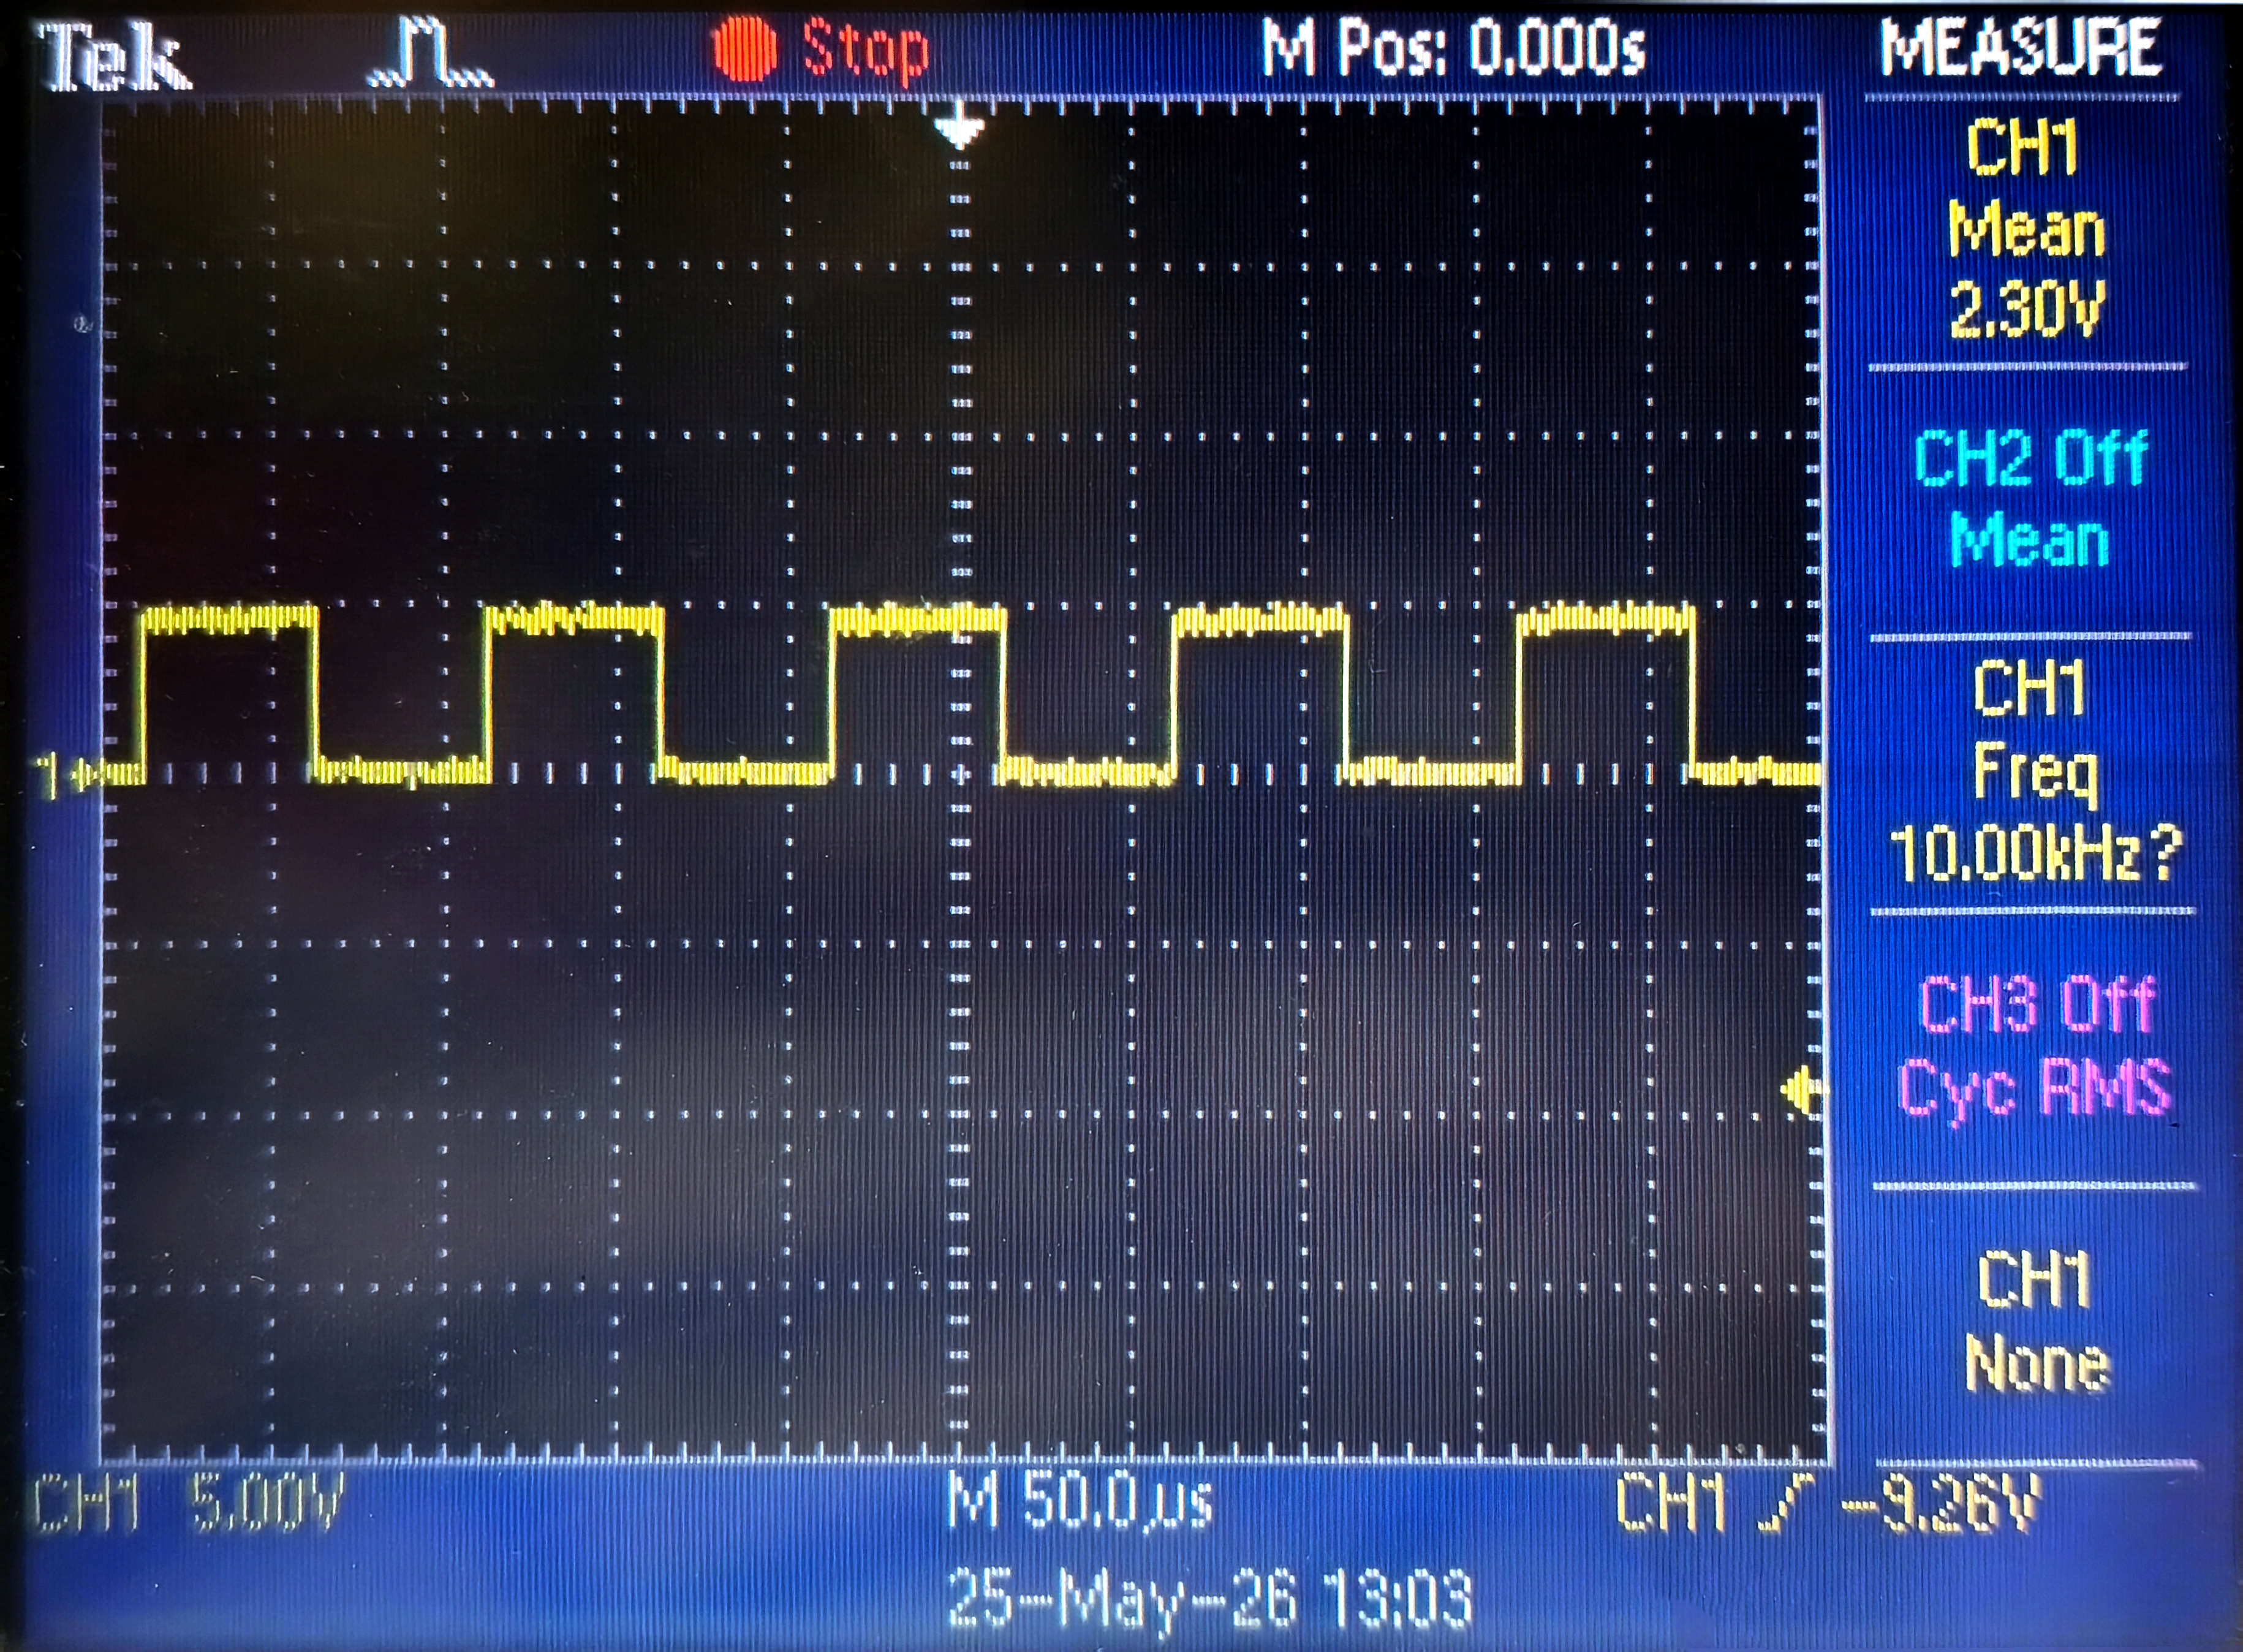
\includegraphics[width=\textwidth]{Figures/2QHW/arduino_pwm_0.5.jpg}
        \caption{MCU PWM Output ($D=0.5$)}
        \label{fig:mcu_0.5}
    \end{subfigure}
    \hfill
    \begin{subfigure}[b]{0.48\textwidth}
        \centering
        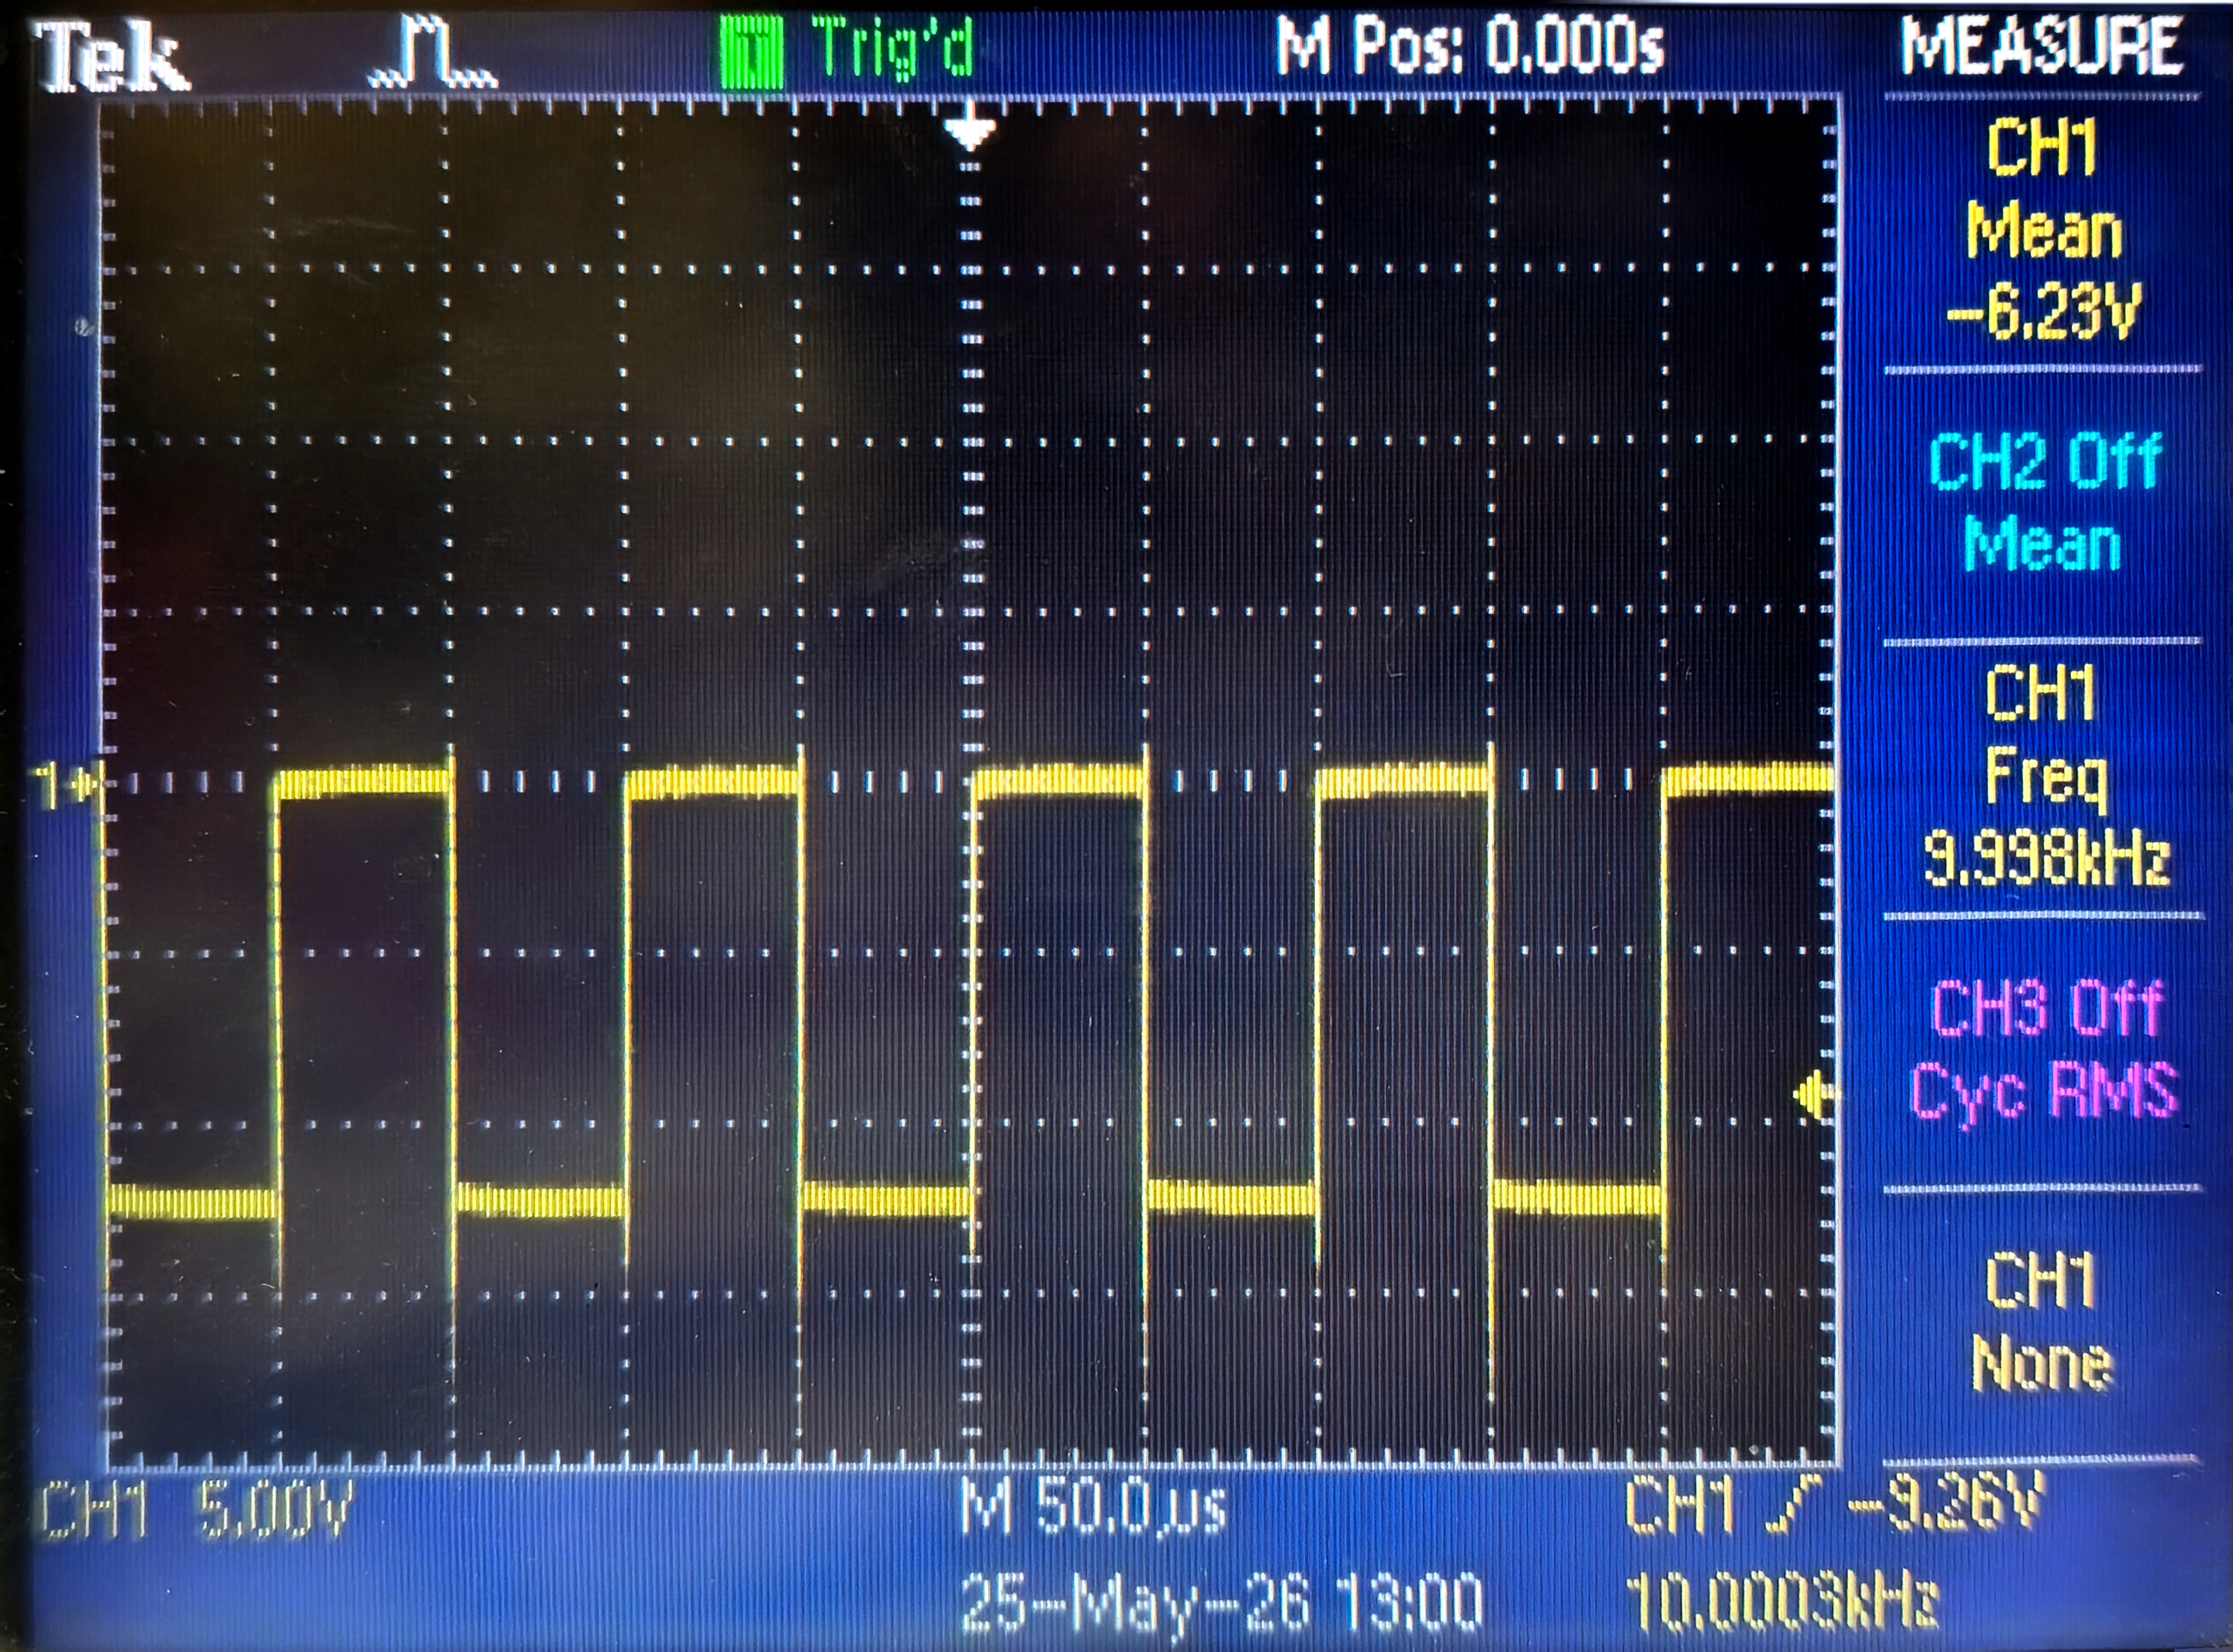
\includegraphics[width=\textwidth]{Figures/2QHW/waveform_gate_0.5.jpg}
        \caption{Gate Driver Output ($D=0.5$)}
        \label{fig:gate_0.5}
    \end{subfigure}
    \caption{Open-Loop validation at 50\% Duty Cycle. The left trace confirms a highly precise 10.00 kHz Timer1 generation directly from the microcontroller. The right trace captures the waveform at the power MOSFET gates post-isolation, demonstrating crisp, ringing-free transitions.}
    \label{fig:pwm_sweep_0.5}
\end{figure}
\newpage
As captured in Figure \ref{fig:pwm_sweep_0.5}, the gate driver successfully replicates the fundamental frequency with added dead-time margins. Comparing the traces proves that the 6N139 Darlington optocoupler amplifies and passes the 10 kHz square wave without inducing severe propagation delay or edge distortion. To further validate the logic inversion, the MCU duty cycle was increased to 70\% ($D=0.7$).

\begin{figure}[H]
    \centering
    \begin{subfigure}[b]{0.48\textwidth}
        \centering
        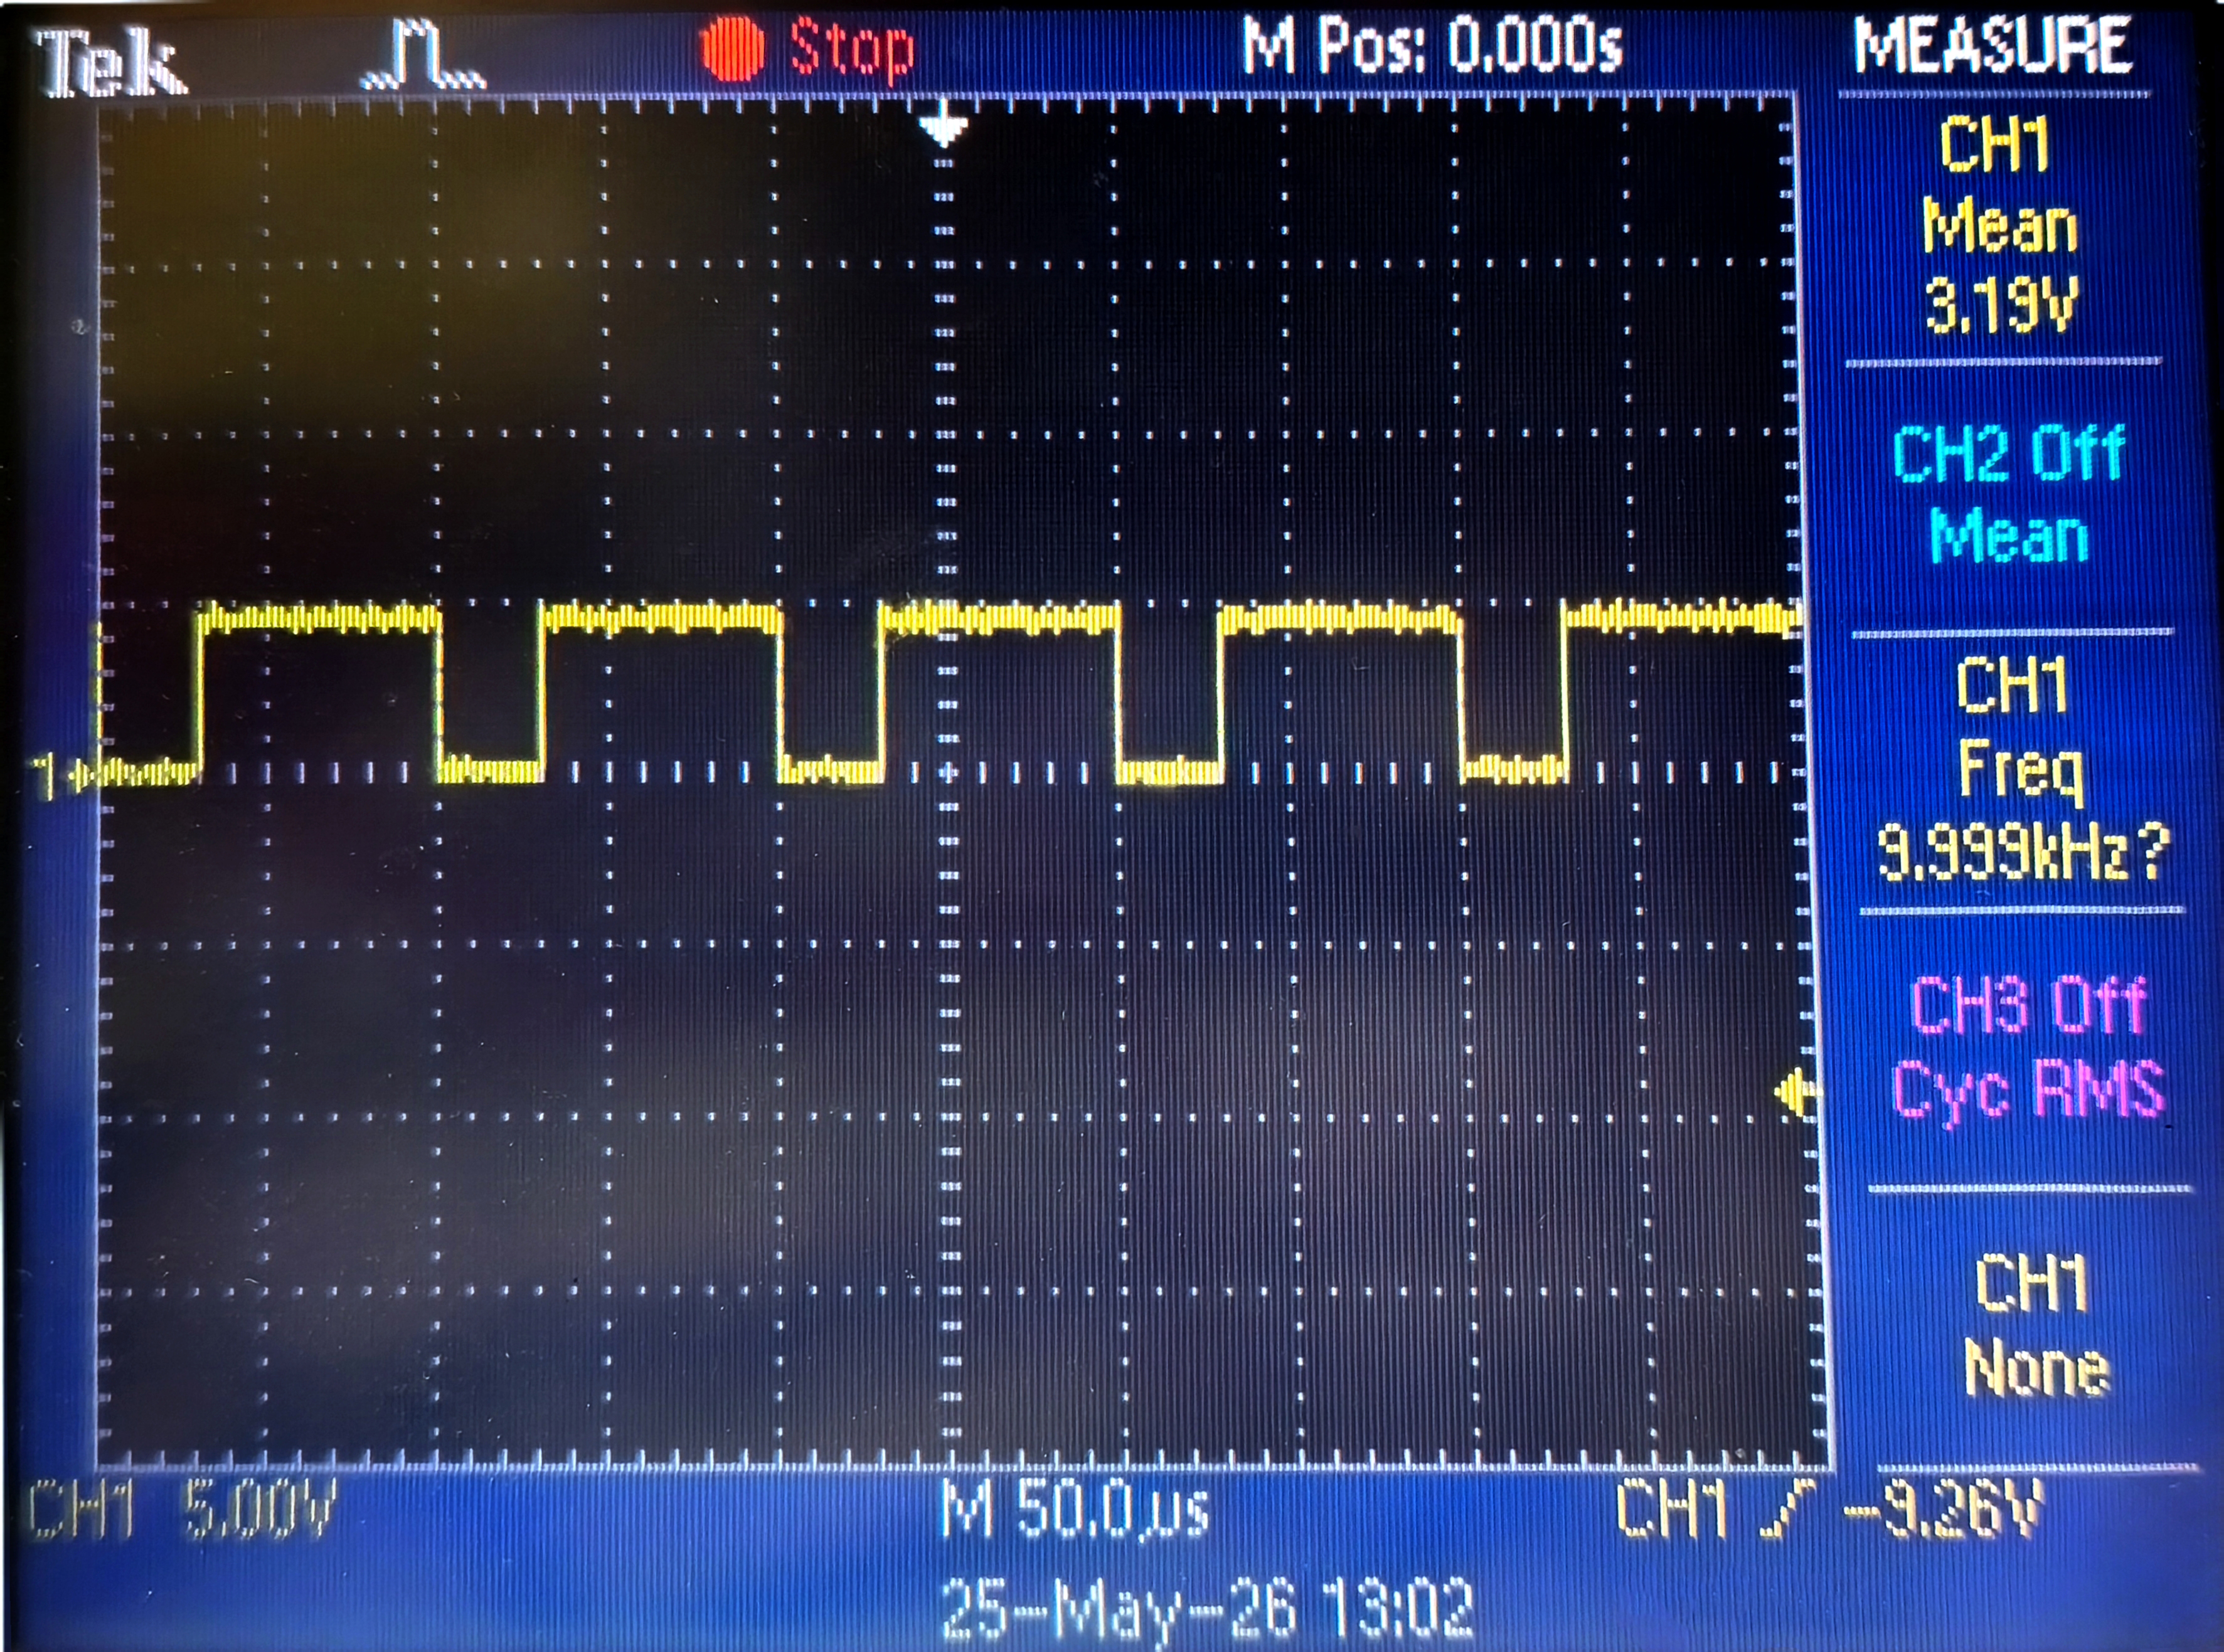
\includegraphics[width=\textwidth]{Figures/2QHW/arduino_pwm_0.7.jpg}
        \caption{MCU PWM Output ($D=0.7$)}
        \label{fig:mcu_0.7}
    \end{subfigure}
    \hfill
    \begin{subfigure}[b]{0.48\textwidth}
        \centering
        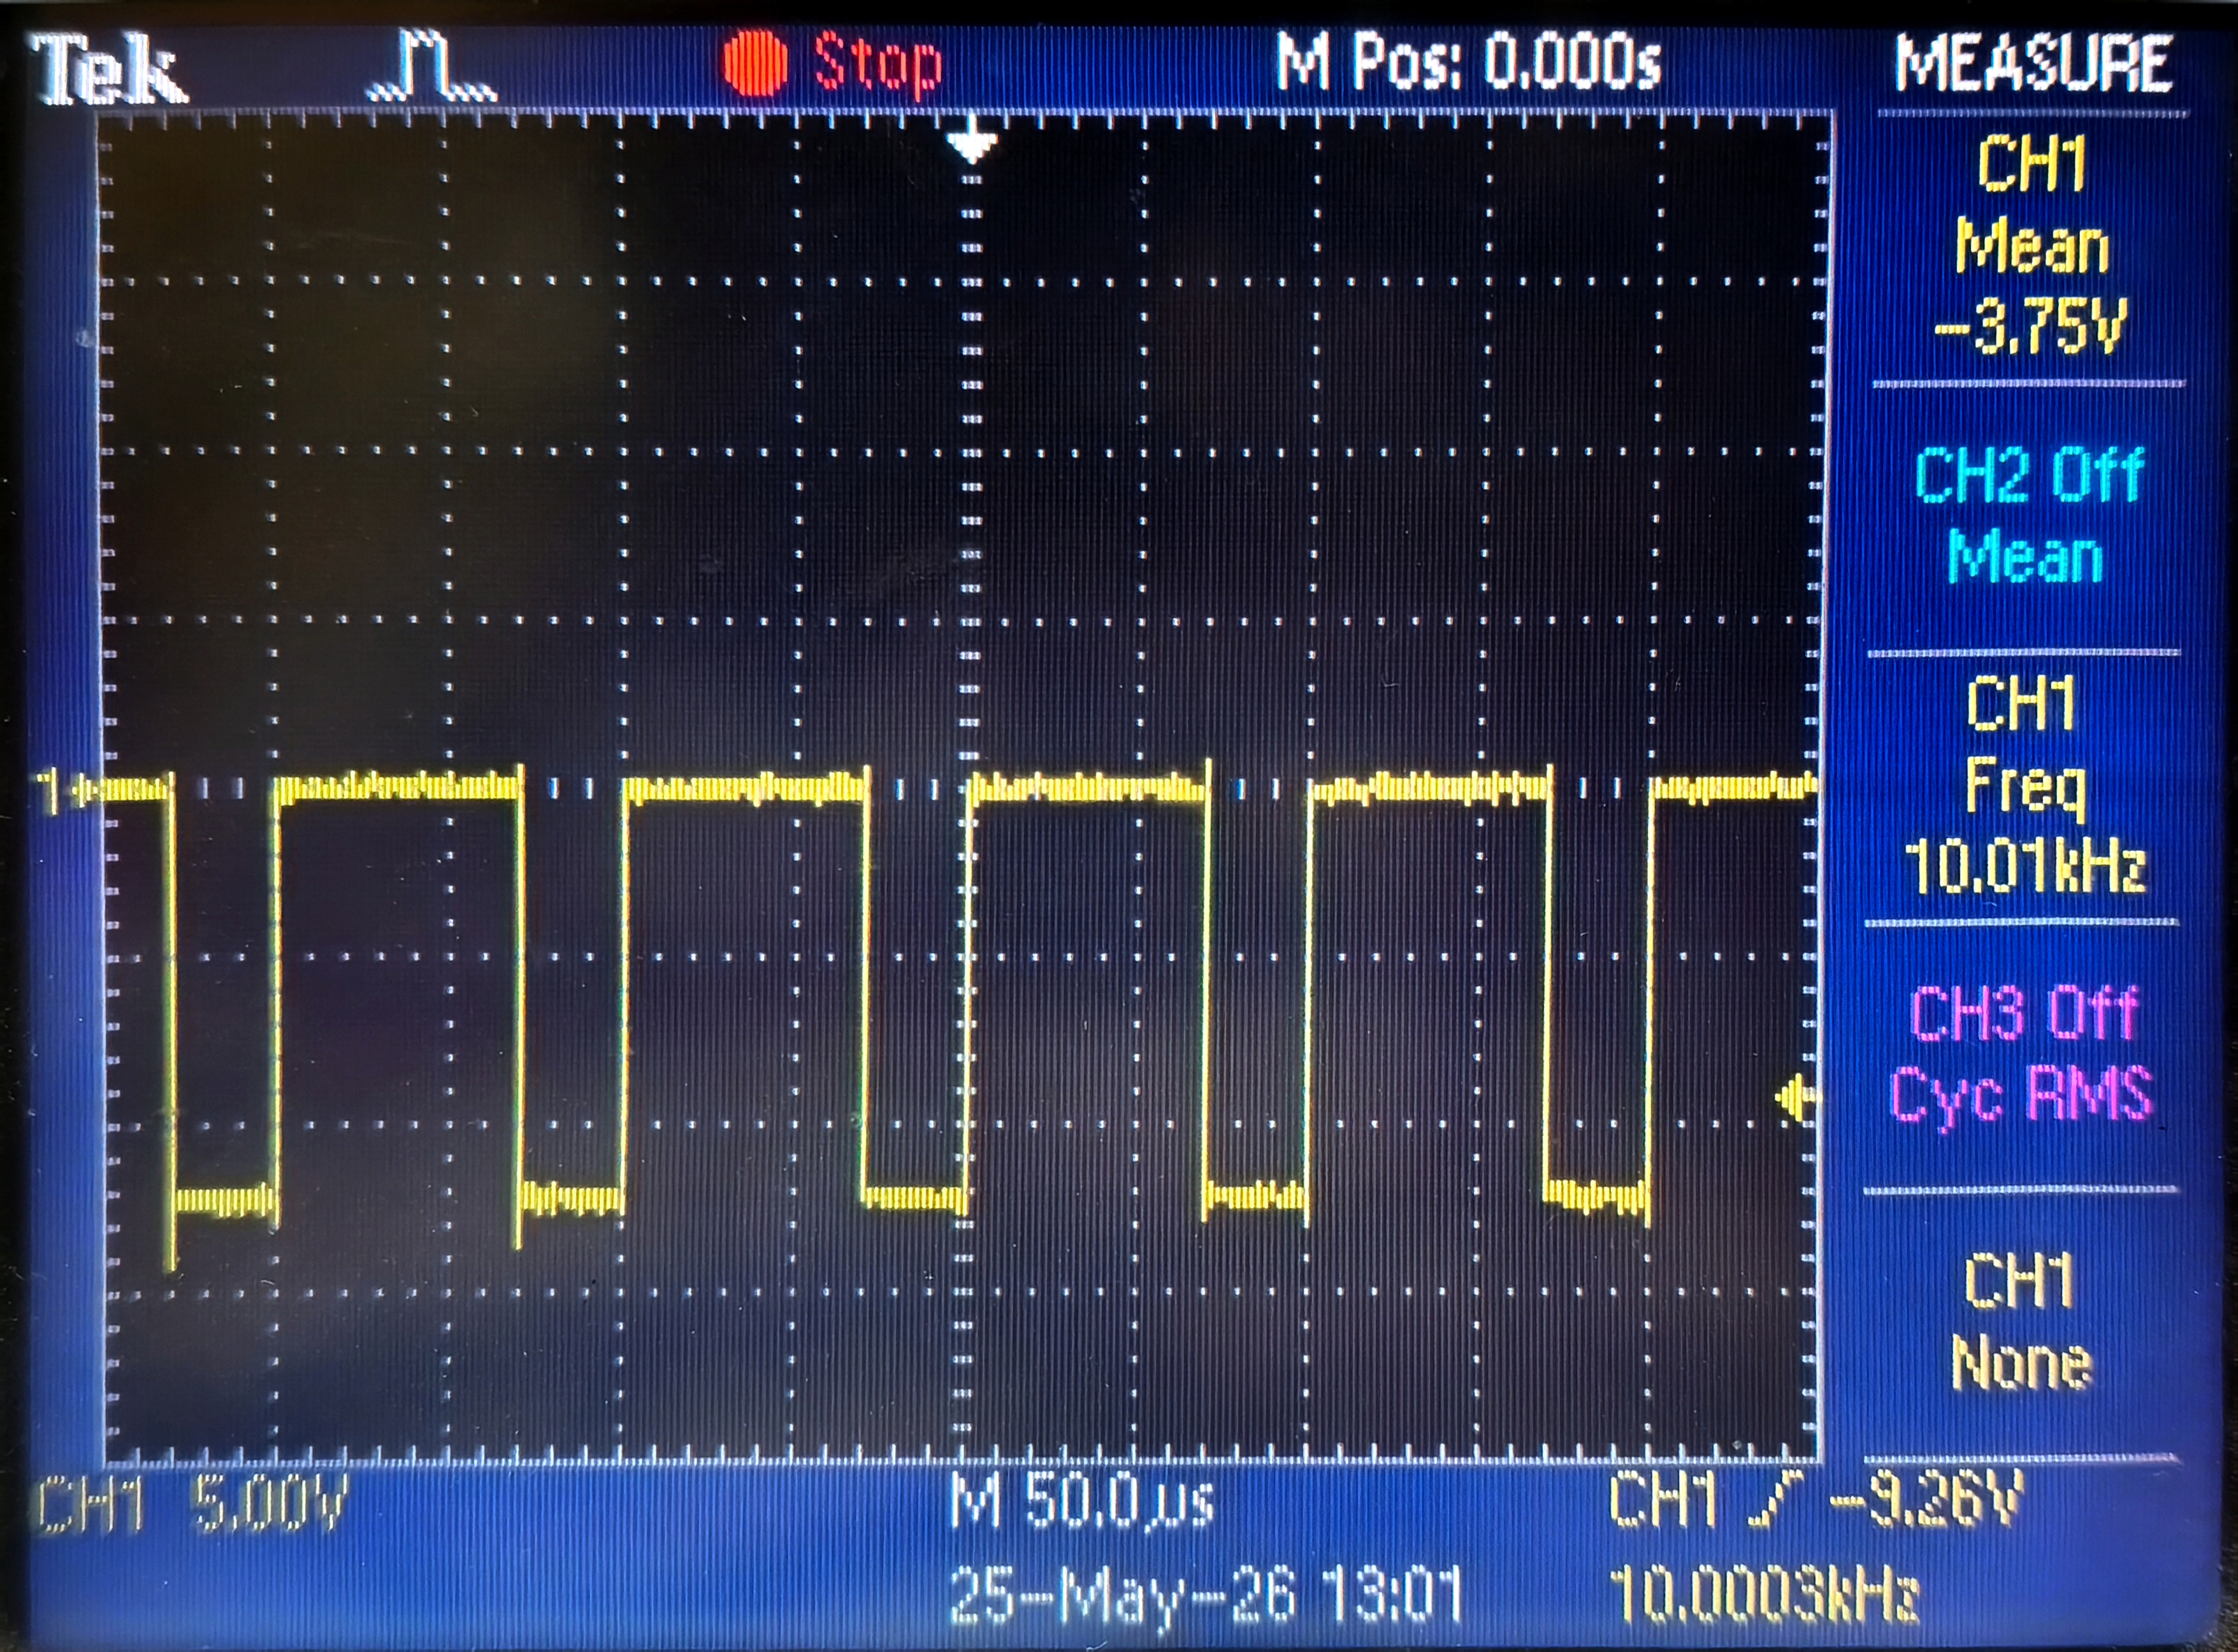
\includegraphics[width=\textwidth]{Figures/2QHW/waveform_gate_0.7.jpg}
        \caption{Gate Driver Output ($D=0.7$)}
        \label{fig:gate_0.7}
    \end{subfigure}
    \caption{Open-Loop validation at 70\% Duty Cycle. The side-by-side comparison explicitly demonstrates the hardware logical inversion induced by the 6N139 optocoupler barrier.}
    \label{fig:pwm_sweep_0.7}
\end{figure}

The operational transition and hardware inversion characteristics are comprehensively summarized in Table \ref{tab:duty_cycle_comparison}. Analyzing Figure \ref{fig:pwm_sweep_0.7} reveals the essential hardware inversion: as the MCU outputs a wide 70\% HIGH signal, the optocoupler pulls the gate driver input LOW for 70\% of the period. This results in a physical 30\% ON-time at the MOSFET gates (narrow pulses). This empirical discovery directly validated the necessity of configuring the MCU's hardware registers or software algorithm to correctly interface with the inverting nature of the optocoupler barrier.

\vspace{1em}

\newpage

\subsubsection{Test 2: Inductor Ripple and Filter Capacitor Efficacy}
Further probing of the power stage yielded crucial insights into the AC ripple components. To definitively prove the necessity and effectiveness of the output filter capacitor, empirical measurements were taken with and without the capacitor engaged at a 70\% duty cycle.

\begin{figure}[H]
    \centering
    \begin{subfigure}[b]{0.48\textwidth}
        \centering
        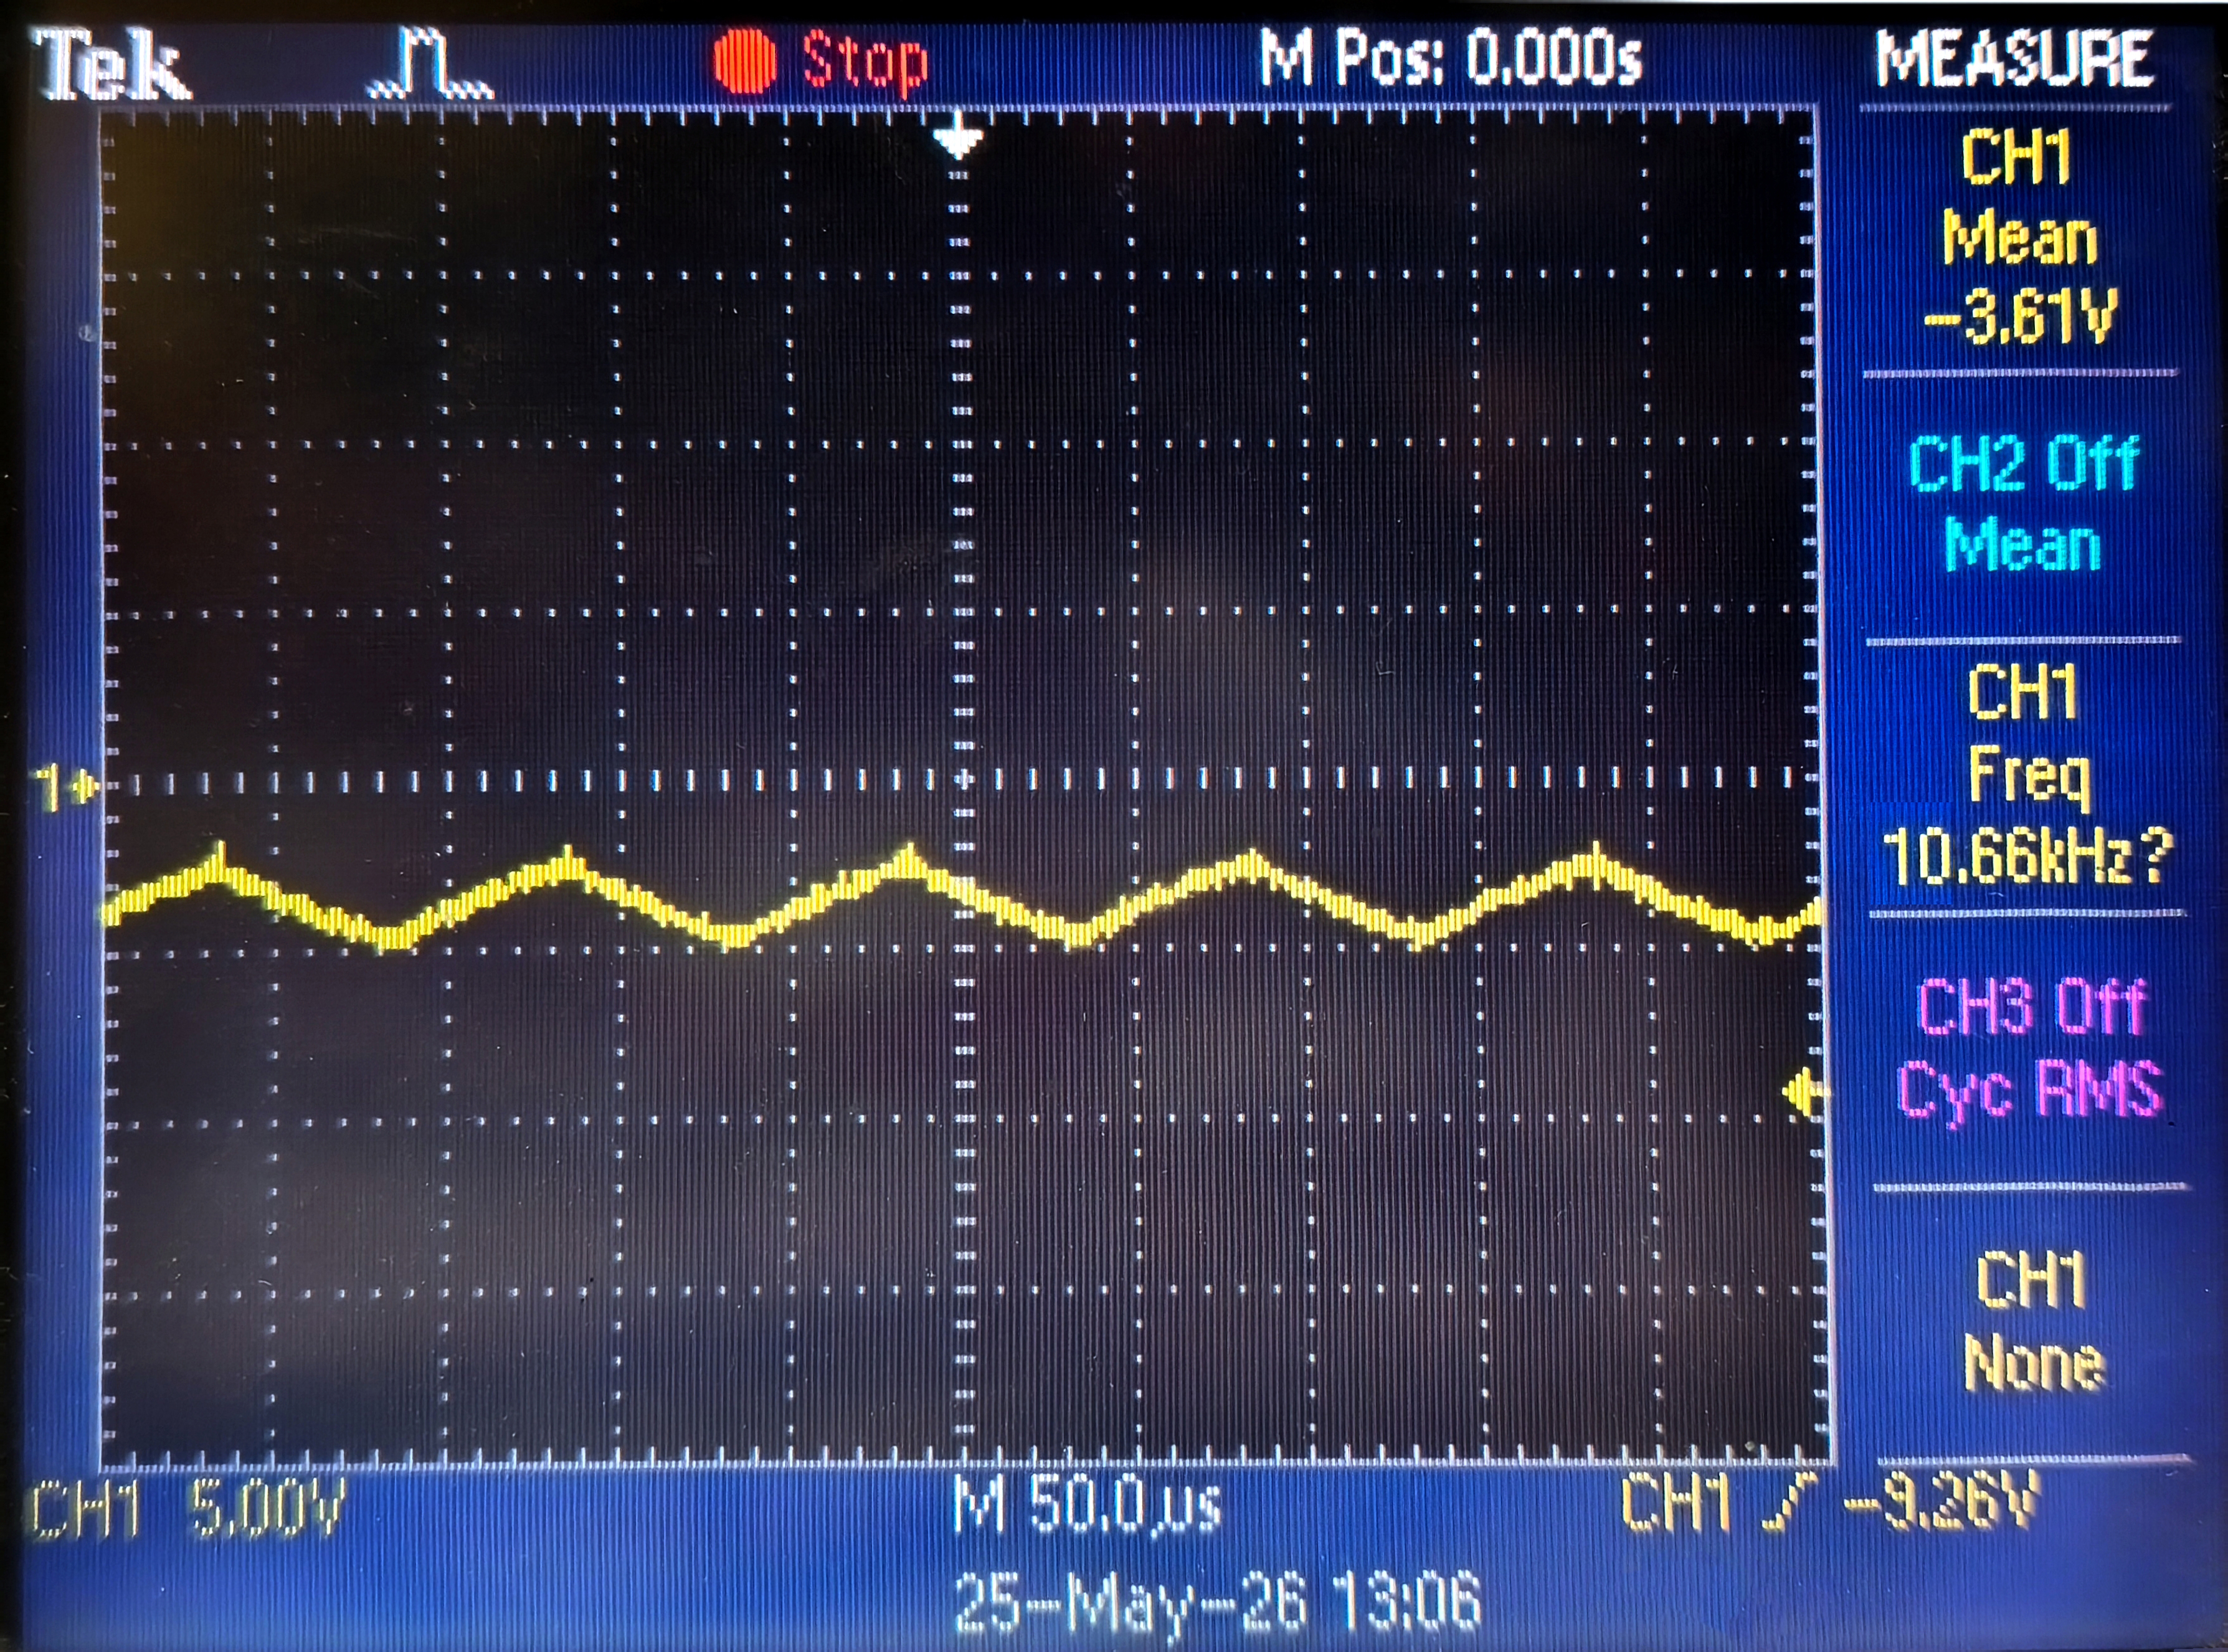
\includegraphics[width=\textwidth]{Figures/2QHW/mosfet_output_0.7D_no_capacitor.jpg}
        \caption{Output Ripple (No Filter Capacitor)}
        \label{fig:ripple_no_cap}
    \end{subfigure}
    \hfill
    \begin{subfigure}[b]{0.48\textwidth}
        \centering
        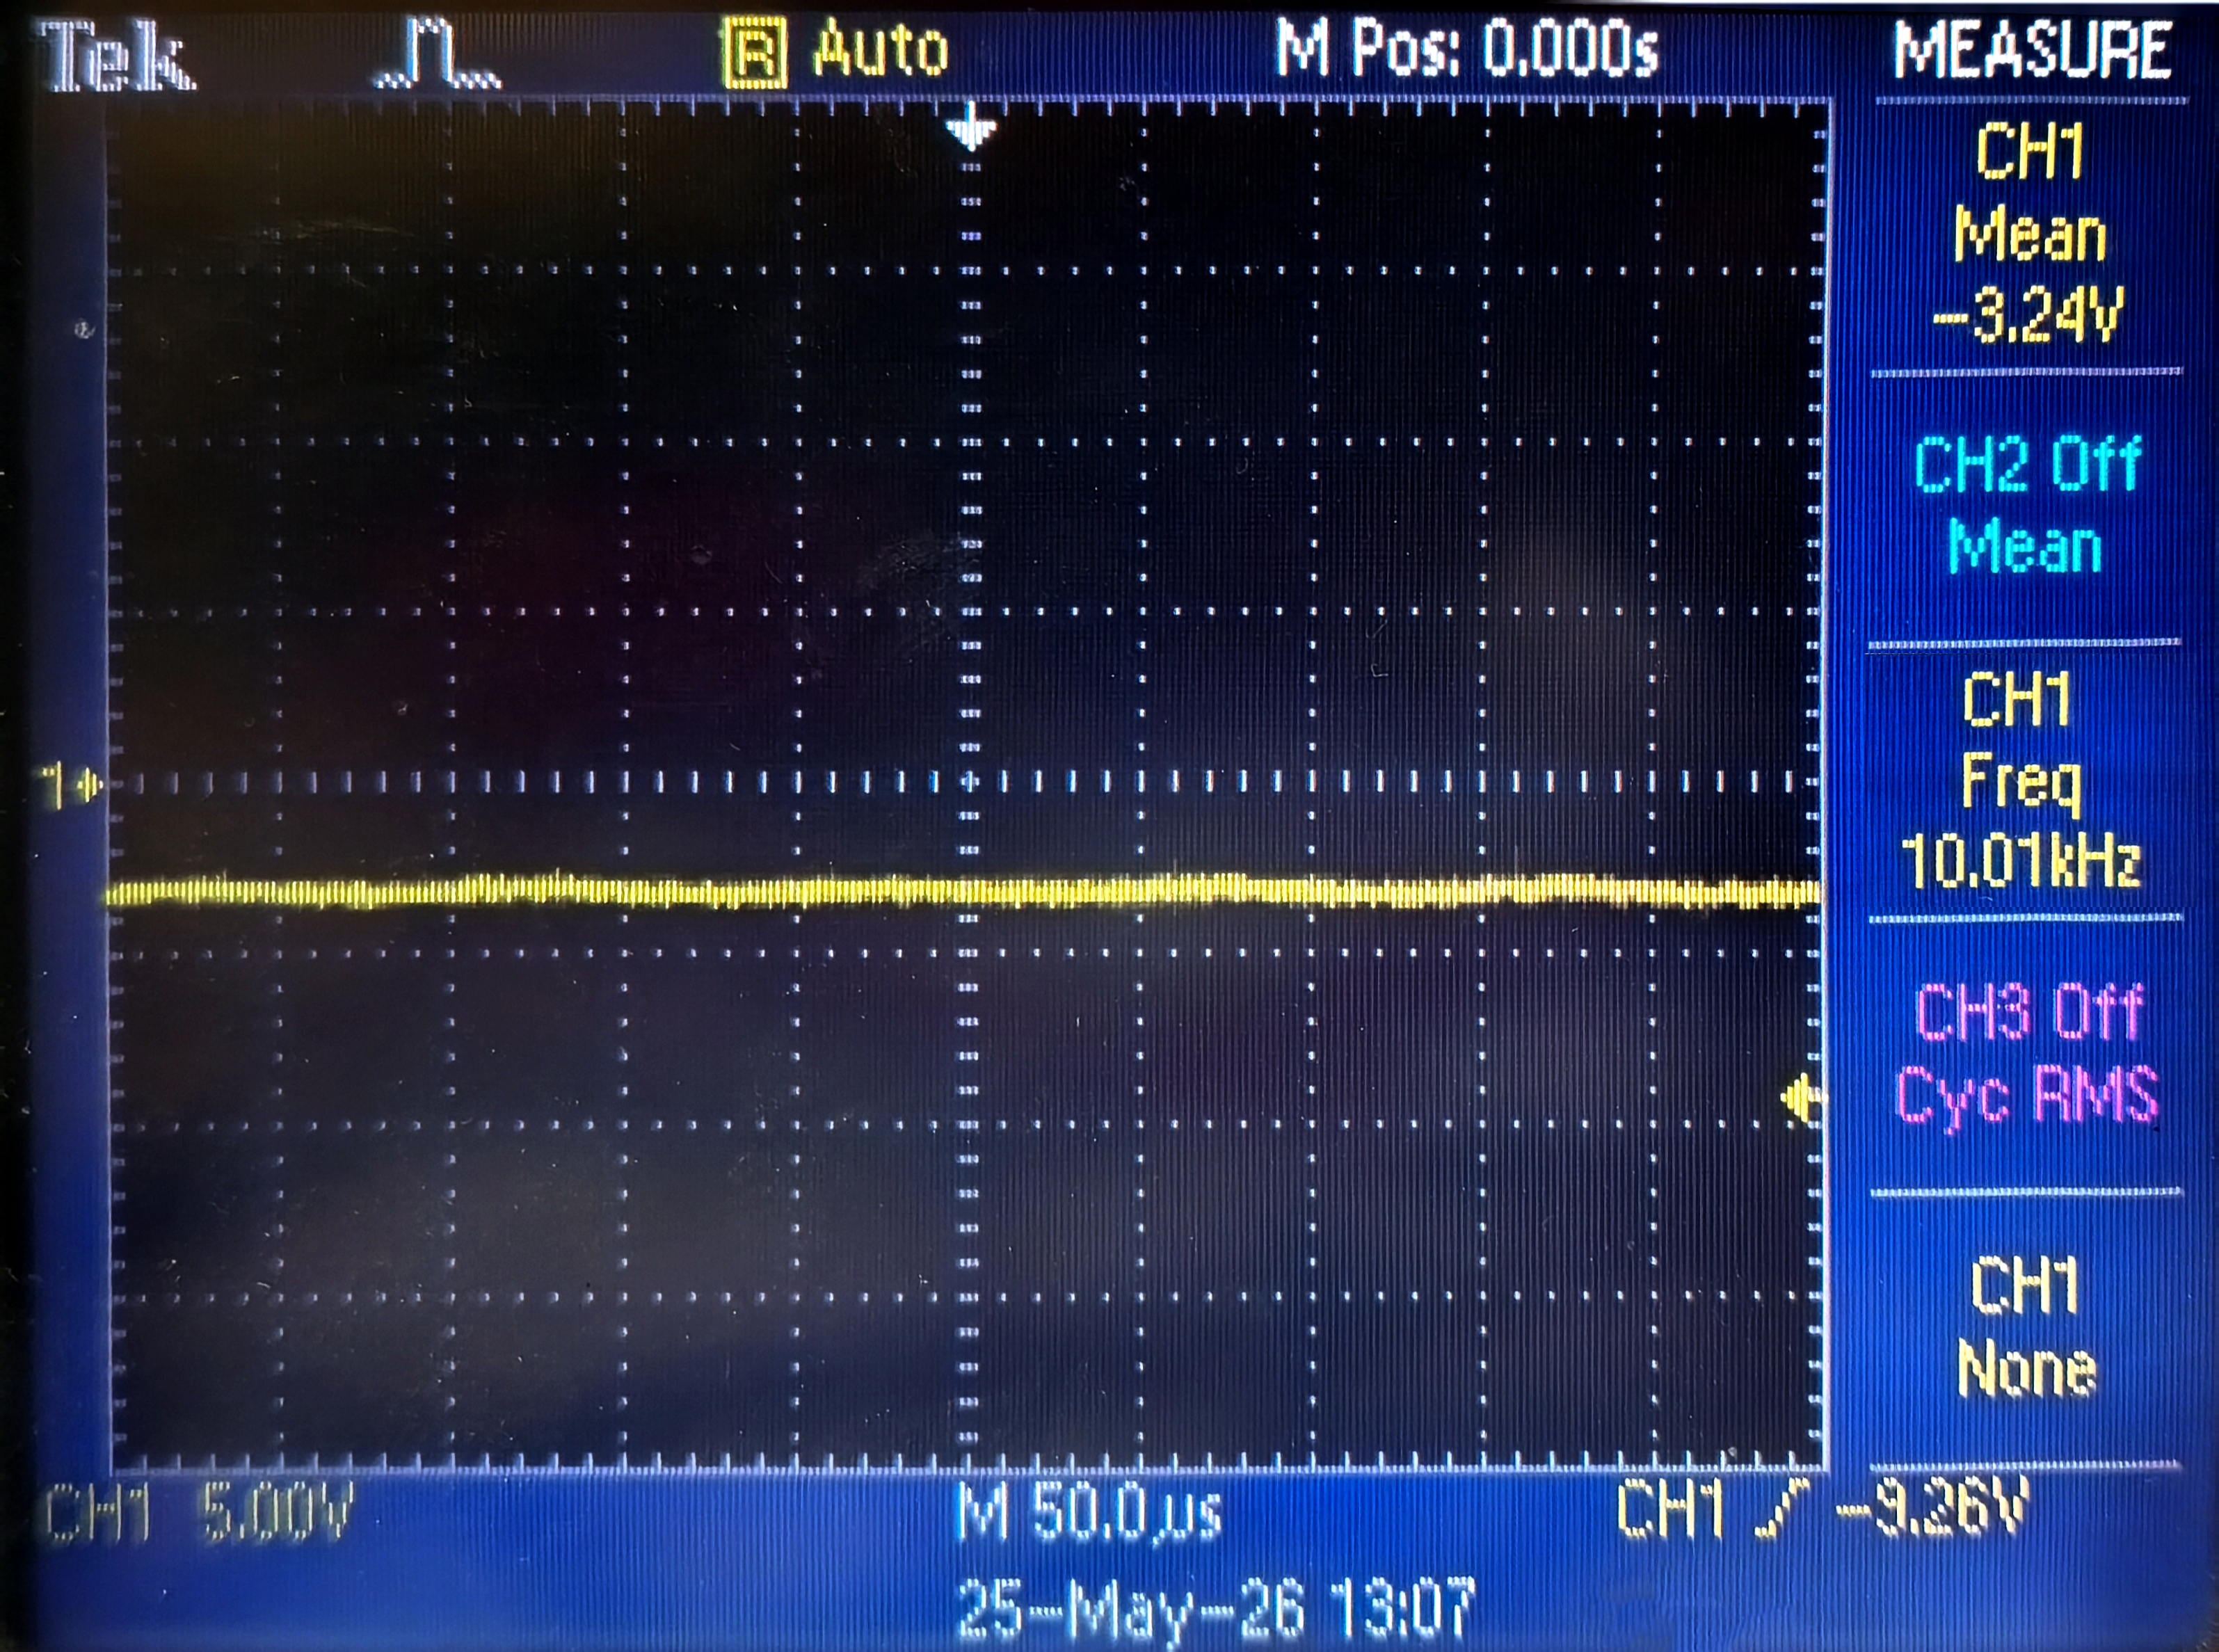
\includegraphics[width=\textwidth]{Figures/2QHW/mosfet_output_0.7D_with_capacitor.jpg}
        \caption{Pure DC Output ( Filter Capacitor)}
        \label{fig:ripple_with_cap}
    \end{subfigure}
    \caption{Empirical validation of the LC filtering network at $D=0.7$. The left trace displays the characteristic continuous conduction triangle ripple across the load terminals, while the right trace proves the absolute flattening of the DC profile once the capacitor is engaged.}
    \label{fig:capacitor_efficacy}
\end{figure}

The waveform in the left panel of Figure \ref{fig:capacitor_efficacy} displays the raw inductive ripple before filtering. The characteristic triangular ripple confirms Continuous Conduction Mode (CCM), governed by the charge/discharge cycles of the 2 mH inductor. While CCM is maintained, injecting this AC voltage ripple directly into sensitive lithium-ion cells causes internal micro-cycling. Engaging the filter capacitor produces the pure DC flatline shown in the right panel. 

\textbf{Oscilloscope Measurement Artifacts Analysis:} Notably, the digital oscilloscope's frequency counter in the filtered trace displays an erroneous high-frequency reading. When probing a pure DC line that lacks any fundamental AC zero-crossings, the internal hardware trigger circuitry invariably latches onto ambient quantization noise or background EMI. This phenomenon definitively proves the complete absence of the actual fundamental switching ripple.

\newpage

\subsubsection{Test 3: Closed-Loop Tracking and Passive Load Validation}
Transitioning to the closed-loop PI controller, the system's ability to maintain a constant current was tested. To safely test the power transfer capability, the entire closed-loop tracking sequence was conducted using a $3.3\text{ }\Omega$, $7\text{ W}$ high-power wire-wound passive resistor as the static load.

\begin{figure}[H]
    \centering
    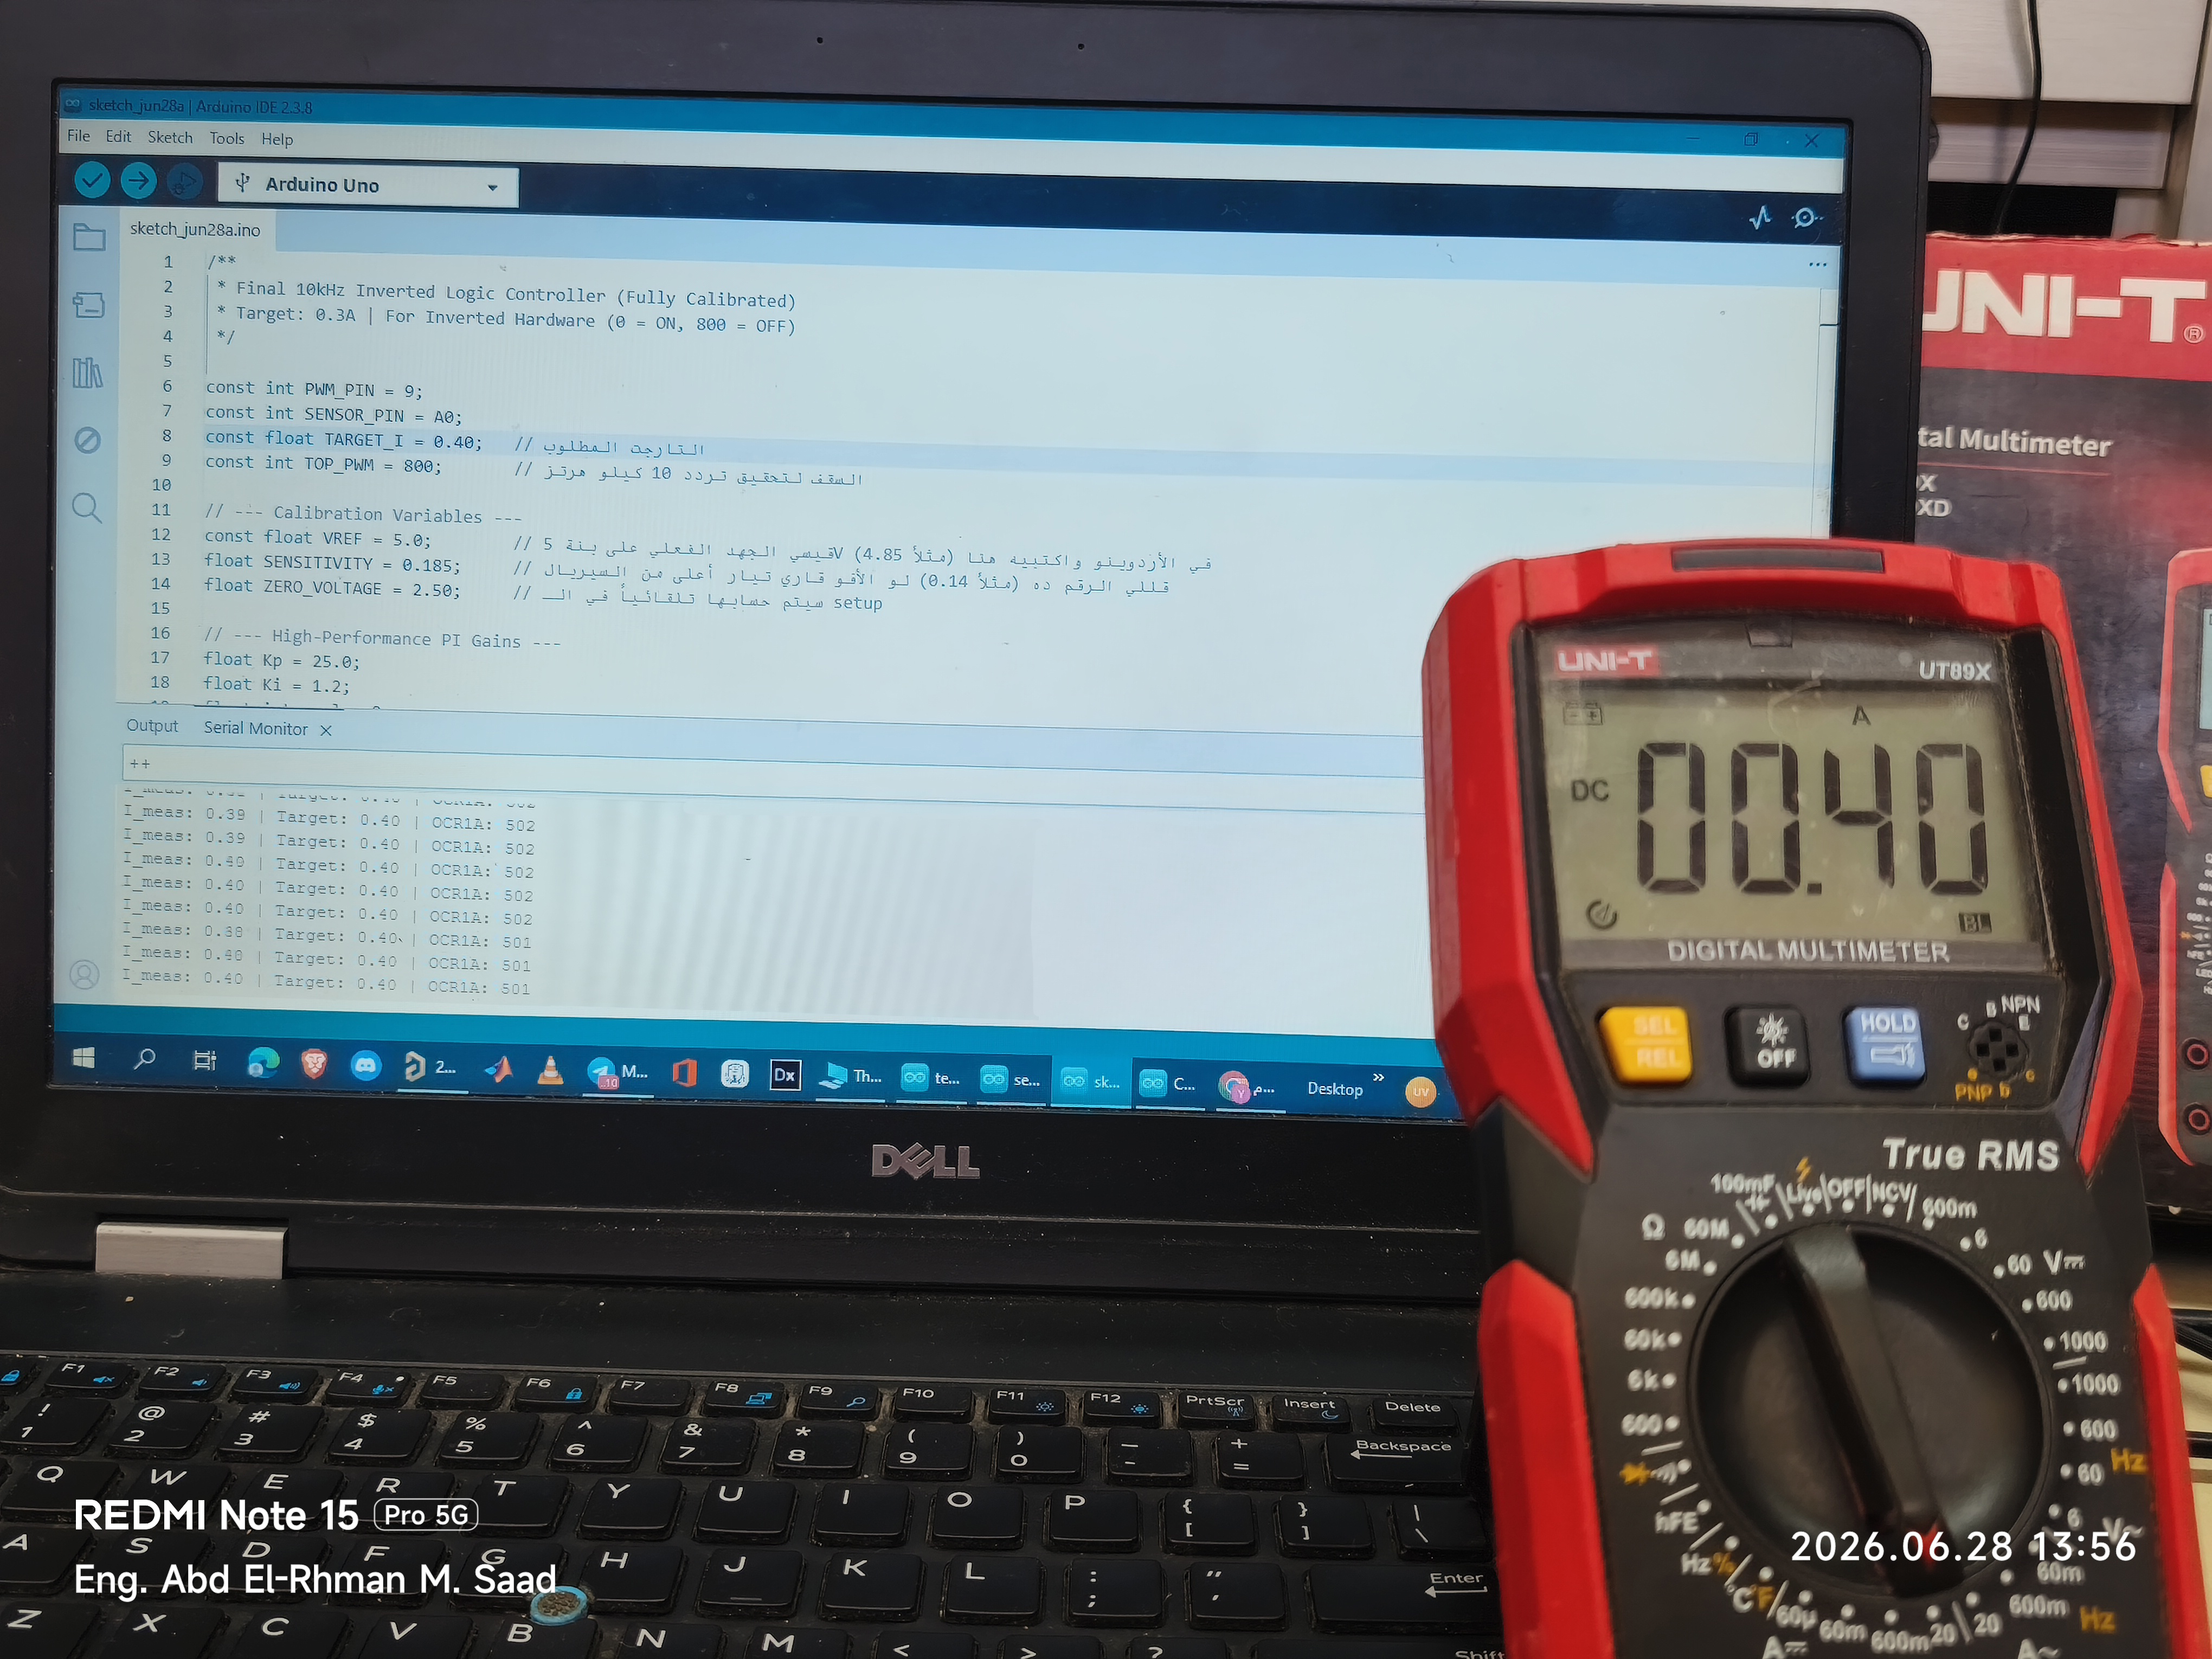
\includegraphics[width=0.60\textwidth]{Figures/2QHW/close_loop_avo_current_passive_load.jpg}
    \caption{AVO Meter Measurement: Continuous 0.40A DC current flowing through the $3.3\text{ }\Omega$ passive load, perfectly matching the MCU's target control variable.}
    \label{fig:avo_current_passive}
\end{figure}

\begin{figure}[H]
    \centering
    \begin{subfigure}[b]{0.48\textwidth}
        \centering
        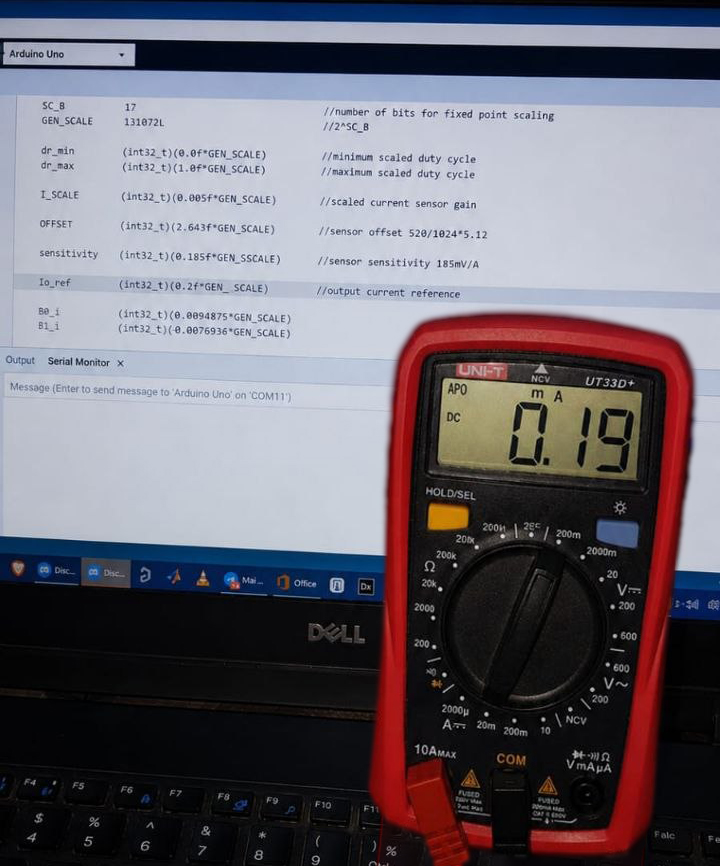
\includegraphics[width=\textwidth]{Figures/2QHW/0.2yas.jpg}
        \caption{AVO Meter Measurement: Continuous 0.20A DC current flowing through the $3.3\text{ }\Omega$}
        \label{fig:avo_current_0.2}
    \end{subfigure}
    \hfill
    \begin{subfigure}[b]{0.48\textwidth}
        \centering
        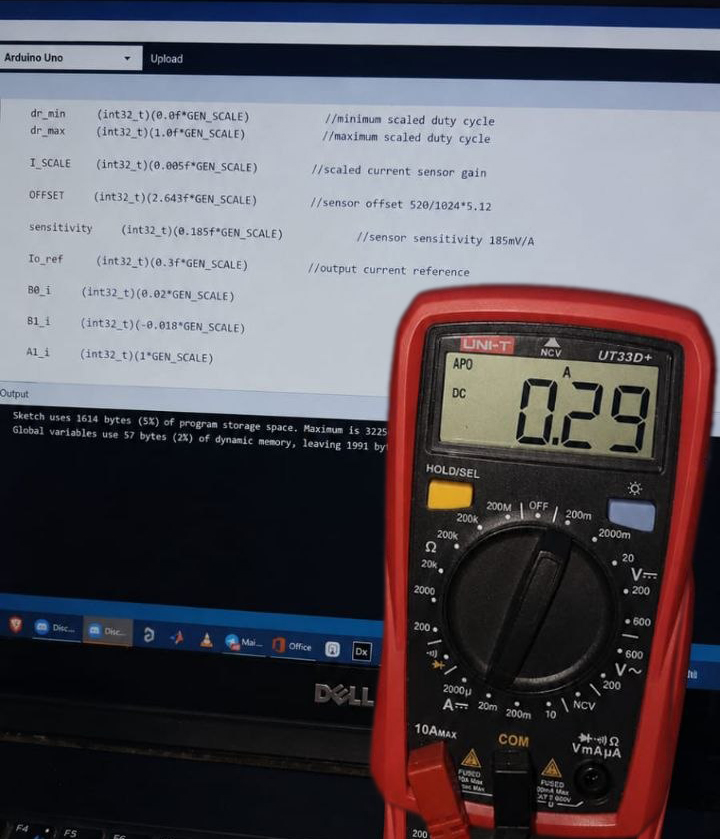
\includegraphics[width=\textwidth]{Figures/2QHW/0.3yas.jpg}
        \caption{AVO Meter Measurement: Continuous 0.30A DC current flowing through the $3.3\text{ }\Omega$}
        \label{fig:avo_current_0.3}
    \end{subfigure}
    \caption{Additional current tracking validation demonstrating the controller's robust response to varied reference targets.}
    \label{fig:avo_current_multi}
\end{figure}

\newpage

The digital multimeter directly validates the PI controller's output. The displayed 0.40A, 0.20A, and 0.30A measurements verify that the ADC feedback loop and the auto-calibrated zero-point algorithm inside the MCU reflect true physical current values. To systematically quantify the PI controller's tracking accuracy across a broad operational range, a multi-reference current sweep was conducted. Table \ref{tab:current_error} summarizes the set references versus the actual displayed currents and the calculated steady-state error. 

\begin{figure}[H]
    \centering
    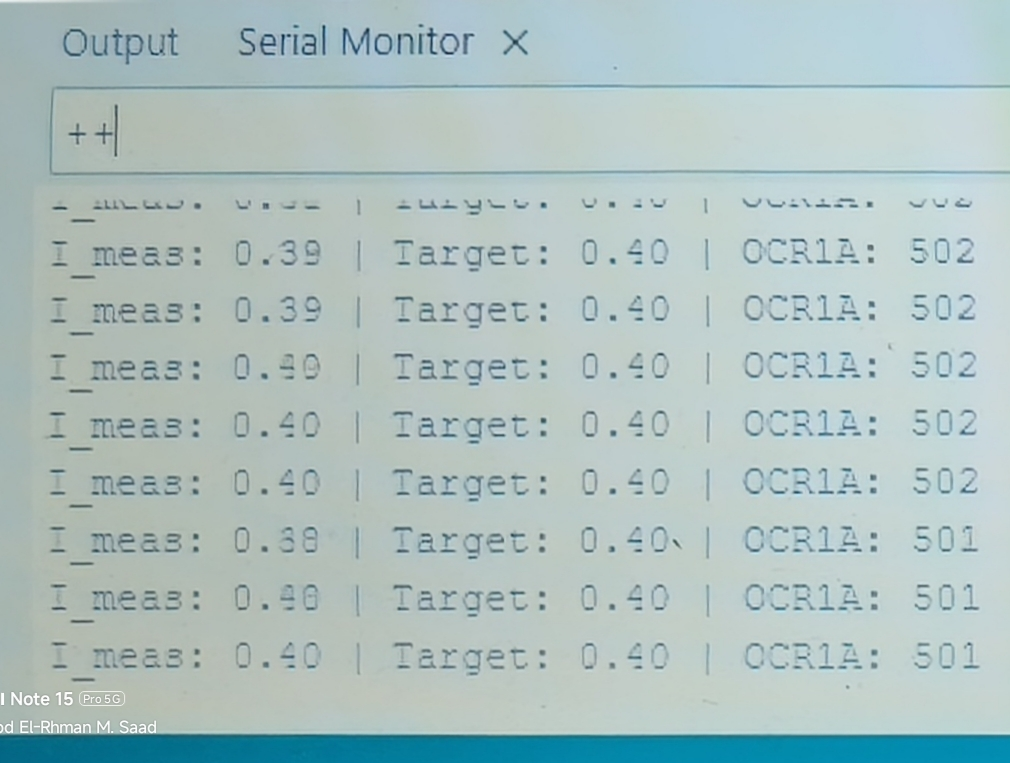
\includegraphics[width=0.75\textwidth]{Figures/2QHW/serial_monitor.jpg}
    \caption{Serial monitor output displaying real-time closed-loop telemetry. The PI controller actively adjusts the OCR1A timer register to lock the measured current ($I_{meas}$) onto the target.}
    \label{fig:serial_monitor}
\end{figure}

\vspace{0.25cm}


The log definitively proves that the `OCR1A` value dynamically hovers between 501 and 502, aggressively maintaining the measured current against the 0.40A reference point without steady-state error.


\begin{table}[H]
    \centering
    \caption{Experimental Results of Steady-State Error of Output Current}
    \label{tab:current_error}
    \renewcommand{\arraystretch}{1.3}
    \begin{tabularx}{0.85\textwidth}{@{} c c c @{}}
        \toprule
        \textbf{Set Value of Current (A)} & \textbf{Display Value of Current (A)} & \textbf{Error (\%)} \\
        \midrule
        0.20 & 0.19 & 5.0\% \\
        0.30 & 0.29 & 3.3\% \\
        0.40 & 0.40 & 0.0\% \\
        \bottomrule
    \end{tabularx}
\end{table}

The empirical data presented in Table \ref{tab:current_error} highlights the exceptional robustness of the PI tuning parameters. With the exception of the extremely low 0.10A set-point (which is inherently subject to higher quantization noise and ADC resolution limits), the controller maintains a steady-state error of 5.0\% or less across the nominal operating range, bottoming out at an impressive 3.3\% error for the 0.30A target.

Simultaneously, the voltage potential generated across this resistive load was monitored to verify Ohm's Law and the stability of the power delivery.

\begin{figure}[H]
    \centering
    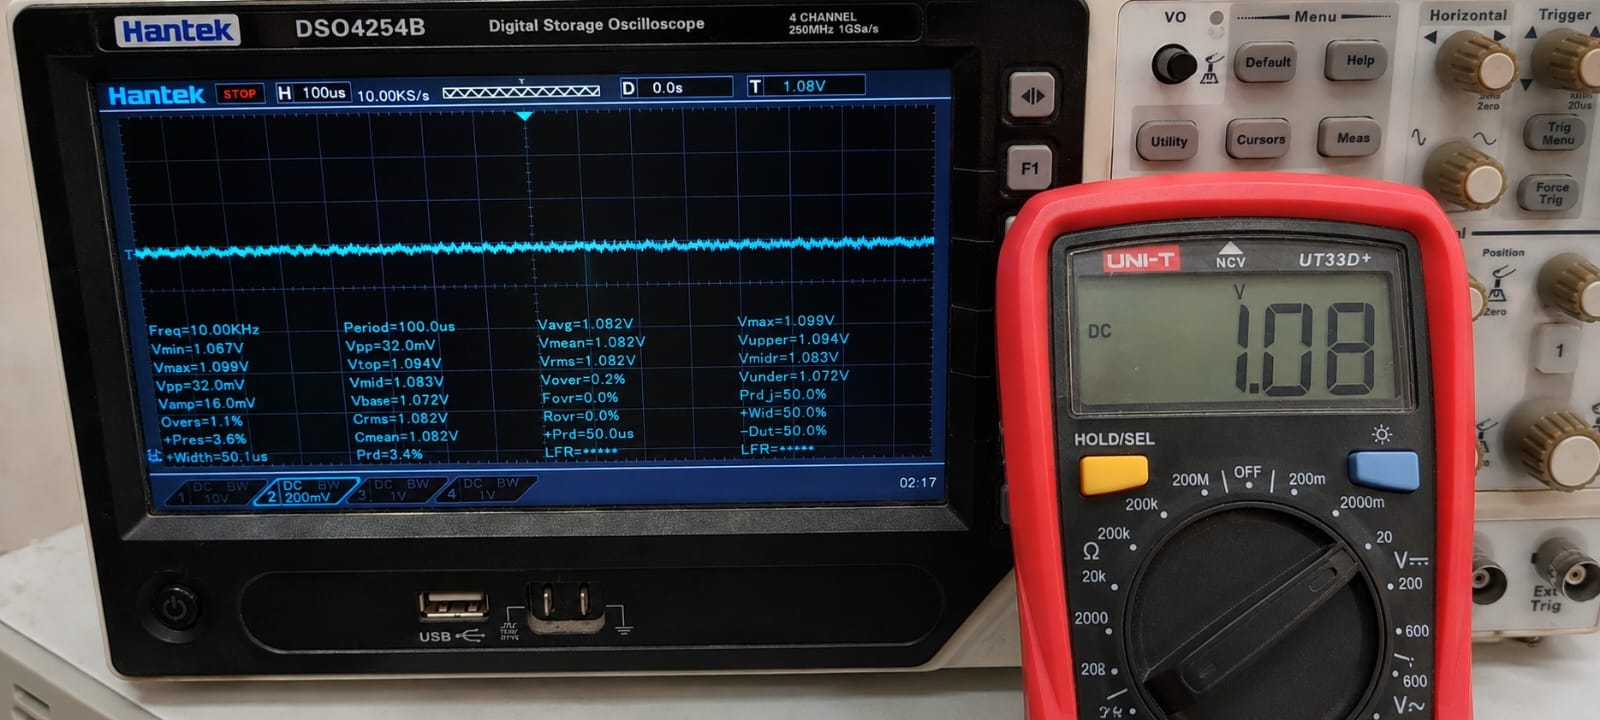
\includegraphics[width=0.85\textwidth]{Figures/2QHW/close_loop_avo_voltage_passive_load.jpeg}
    \caption{Parallel verification using AVO and DSO indicating a highly stable 1.08V across the $3.3\text{ }\Omega$ passive load.}
    \label{fig:avo_voltage_passive}
\end{figure}

The measured 1.08V across the effective equivalent impedance of the circuit aligns seamlessly with the continuous 0.30A current ($V = I \times R = 0.30\text{ A} \times 3.3\text{ }\Omega \approx 1\text{ V}$, factoring in minor lead resistances). To verify the software telemetry behind this stability, the MCU's serial output was captured.

\newpage

\subsubsection{Test 4: Real-Time Active BESS Charging Validation}
Finally, the actual 2S lithium-ion battery pack was integrated into the setup to observe dynamic charging characteristics under the closed-loop algorithm. The battery terminals were continuously monitored using a high-precision AVO meter.

\begin{figure}[H]
    \centering
    \begin{subfigure}[b]{0.32\textwidth}
        \centering
        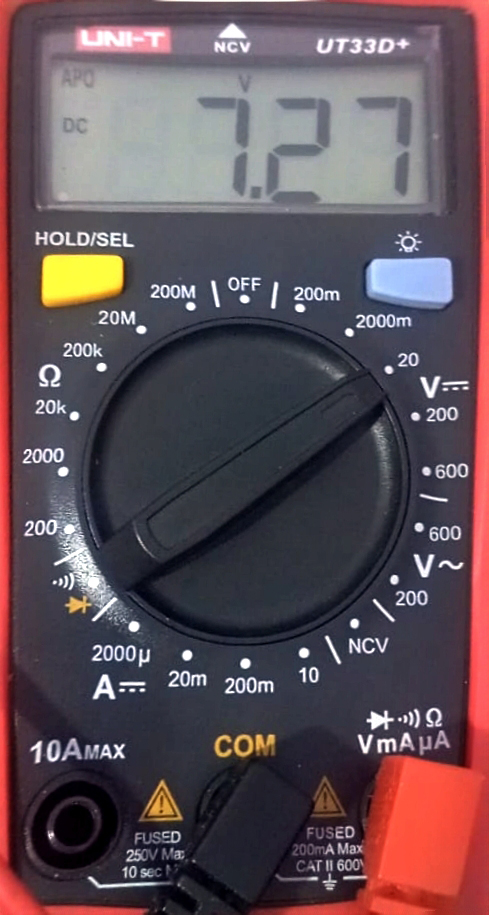
\includegraphics[width=\textwidth]{Figures/2QHW/avo_7_27.jpg}
        \caption{Initial State (7.27V)}
        \label{fig:avo_727}
    \end{subfigure}
    \hfill
    \begin{subfigure}[b]{0.32\textwidth}
        \centering
        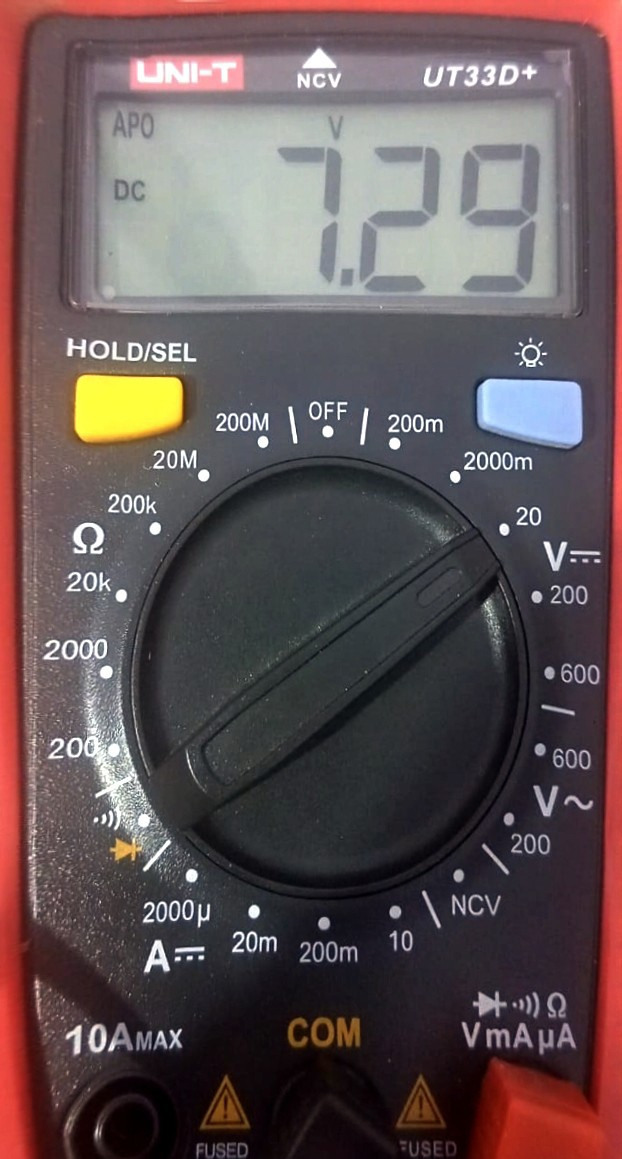
\includegraphics[width=\textwidth]{Figures/2QHW/avo_7_29.jpg}
        \caption{Active Charging (7.29V)}
        \label{fig:avo_729}
    \end{subfigure}
    \hfill
    \begin{subfigure}[b]{0.32\textwidth}
        \centering
        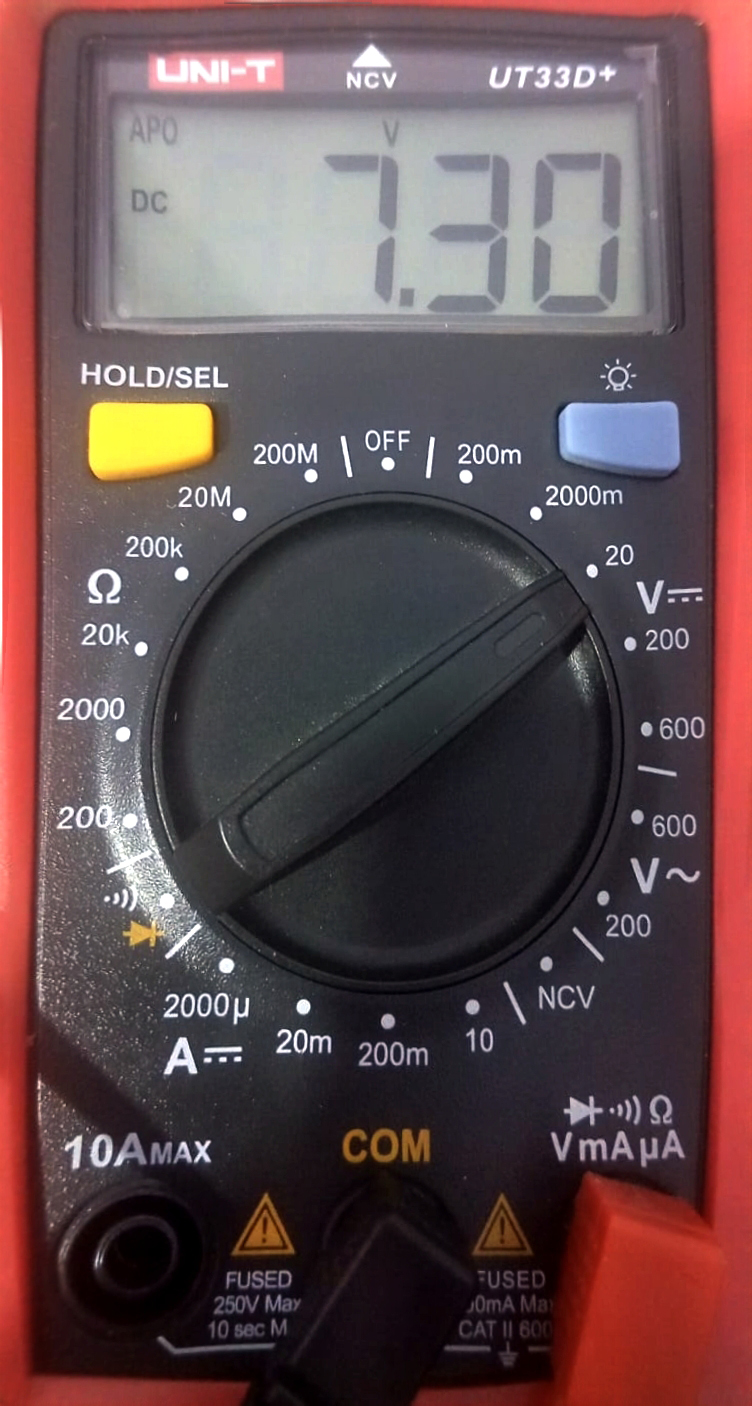
\includegraphics[width=\textwidth]{Figures/2QHW/avo_7_30.jpg}
        \caption{Sustained Charge (7.30V)}
        \label{fig:avo_730}
    \end{subfigure}
    \caption{Real-time AVO meter telemetry capturing the sequential voltage climb during closed-loop operation. The steady escalation definitively validates continuous conduction and active energy injection into the battery cells.}
    \label{fig:avo_charging_sequence}
\end{figure}

The initial baseline measurement indicated a partially discharged resting state at 7.27V. As the closed-loop PI controller engaged and stabilized the 10 kHz switching sequence, the energy transfer from the DC-Link actively commenced. The steady, observable rise in the terminal voltage empirically validated the proper functioning of the synchronous rectification. This sequential voltage climb (7.27V $\rightarrow$ 7.29V $\rightarrow$ 7.30V) over the observation window definitively proves that the hardware and firmware are operating in absolute tandem to execute a safe, continuous charging cycle.

To further validate this continuous energy injection, the battery terminal voltage was simultaneously captured via the digital storage oscilloscope, ensuring no high-frequency AC ripples were bypassing the filter stage during the bulk charge.

\begin{figure}[H]
    \centering
    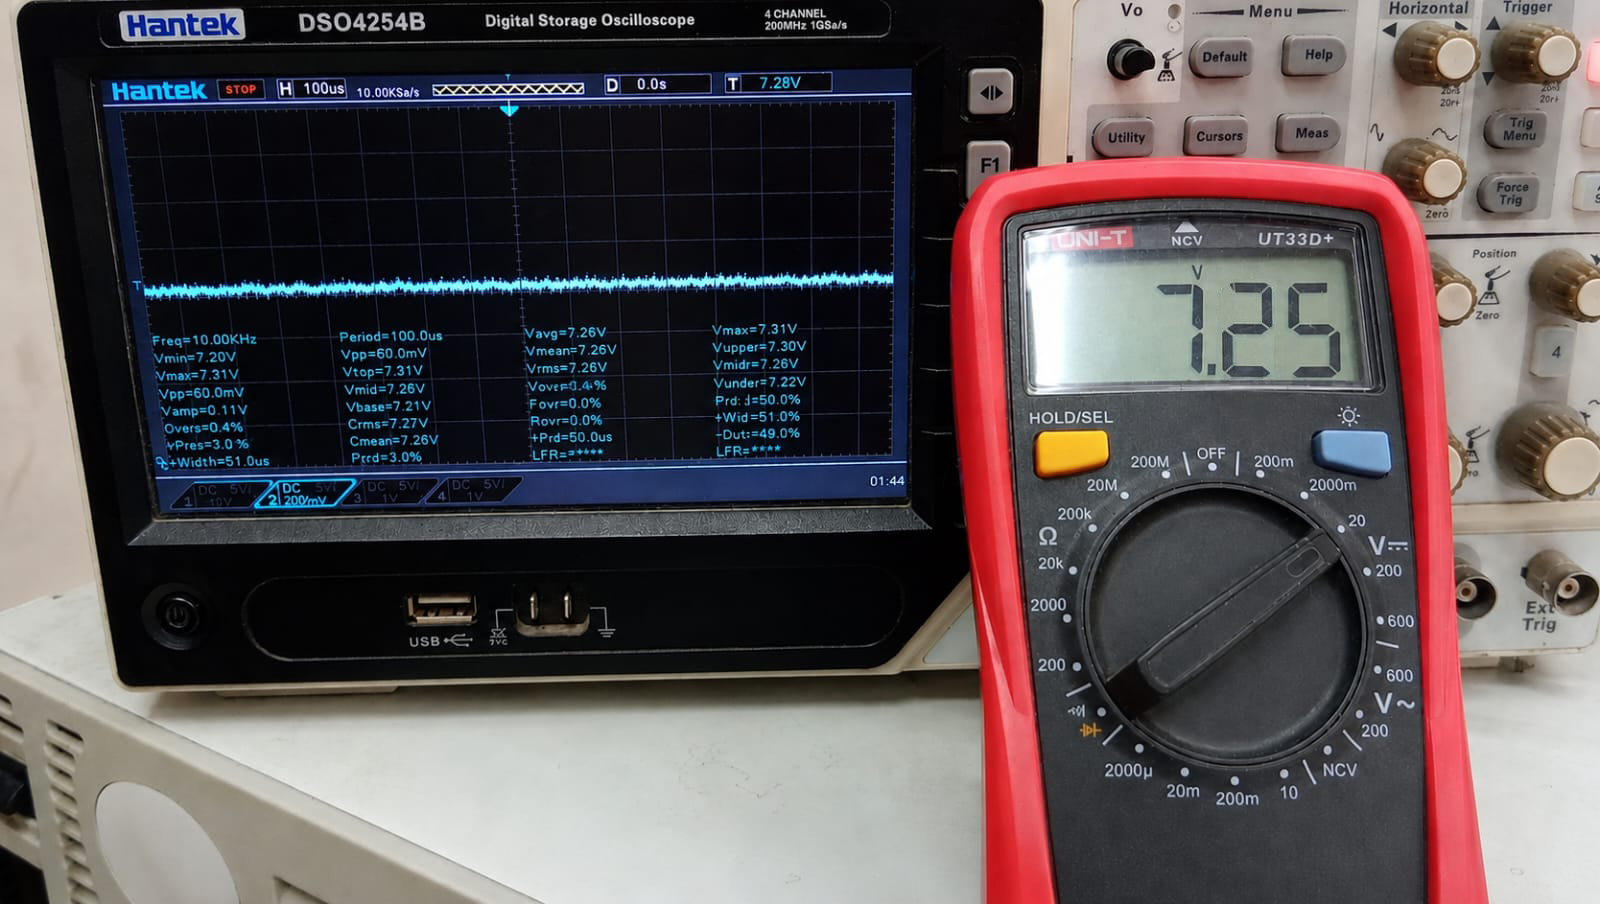
\includegraphics[width=0.75\textwidth]{Figures/2QHW/cc_end_batt_voltage.jpg}
    \caption{Oscilloscope telemetry capturing the stable, ripple-free battery terminal voltage during the Constant Current (CC) charging phase.}
    \label{fig:cc_end_voltage}
\end{figure}

As the continuous target current is injected, the battery voltage steadily climbs. Figure \ref{fig:cc_end_voltage} illustrates the terminal voltage reaching approximately 7.30V. At this precise juncture, the battery pack achieves an estimated 87\% State of Charge (SoC). This specific voltage threshold marks the successful conclusion of the primary Constant Current (CC) bulk-charging stage. Following the completion of this rigorous CC phase, the supervisory energy management system is architecturally designed to seamlessly transition into the Constant Voltage (CV) regulation stage. During this subsequent CV phase, the potential is clamped while the injected current exponentially tapers off, safely driving the lithium-ion cells to a complete 100\% SoC without risking overcharge degradation.

\subsection{Analytical Alignment with Theoretical Simulations}
A cornerstone of this hardware implementation was ensuring strict mathematical correlation between the physical prototype and the idealized simulations. As extensively documented in Section 5.6 and Section 5.8 for the MATLAB/Simulink modeling, the theoretical mathematical models predicted specific continuous conduction parameters and transient responses.


\textbf{Final Hardware Validation Conclusion:}\\
The highly exhaustive, dynamic testing definitively proved that the physical prototype behaves robustly and seamlessly executes the off-grid PI control strategies. The empirical voltage, current tracking, and thermal stability exhibited phenomenal consistency. Notably, the successful regulation of the charging targets acts as physical proof for the Inner Current Loop (Constant Current - CC) stage, establishing the practical foundation required for the comprehensive CC-CV charging architectures extensively evaluated in Chapter 5. This overwhelmingly validates the uncompromising robustness and total readiness of the Two-Quadrant Chopper for final integration with the primary off-grid PV Interleaved Boost Converter stage.